%  LaTeX support: latex@mdpi.com
%  For support, please attach all files needed for compiling as well as the log file, and specify your operating system, LaTeX version, and LaTeX editor.

%=================================================================
\documentclass[journal,article,submit,moreauthors,technologies]{Definitions/mdpi}
%\documentclass[journal,article,submit,moreauthors,unicode]{Definitions/mdpi} % For some letters Palatino lacks
%\documentclass[preprints,article,submit,moreauthors]{Definitions/mdpi}
%\documentclass[preprints,article,submit,moreauthors,unicode]{Definitions/mdpi}
% For posting an early version of this manuscript as a preprint, you may use "preprints" as the journal. Changing "submit" to "accept" before posting will remove line numbers.

%=================================================================
% Class Options:
% journal = technologies
% article = article
% submit = submit (will be changed to accept by Editorial Office)
% moreauthors = more than one author
%=================================================================

%=================================================================
% MDPI internal commands - do not modify
\firstpage{1}
\makeatletter
\setcounter{page}{\@firstpage}
\makeatother
\pubvolume{1}
\issuenum{1}
\articlenumber{0}
\pubyear{2026}
\copyrightyear{2026}
%\externaleditor{Firstname Lastname} % More than 1 editor, please add `` and '' before the last editor name
\datereceived{ }
\daterevised{ } % Comment out if no revised date
\dateaccepted{ }
\datepublished{ }
%\datecorrected{} % For corrected papers: "Corrected: XXX" date in the original paper.
%\dateretracted{} % For retracted papers: "Retracted: XXX" date in the original paper.
%\doinum{} % Used for some special journals, like molbank
%\pdfoutput=1 % Uncommented for upload to arXiv.org
%\CorrStatement{yes}  % For updates
%\longauthorlist{yes} % For many authors that exceed the left citation part
%\IsAssociation{yes} % For association journals

%=================================================================
% Add packages and commands here. The following packages are loaded in our class file: fontenc, inputenc, calc, indentfirst, fancyhdr, graphicx, epstopdf, lastpage, ifthen, float, amsmath, amssymb, lineno, setspace, enumitem, mathpazo, booktabs, titlesec, etoolbox, tabto, xcolor, colortbl, soul, multirow, microtype, tikz, totcount, changepage, attrib, upgreek, array, tabularx, pbox, ragged2e, tocloft, marginnote, marginfix, enotez, amsthm, natbib, hyperref, cleveref, scrextend, url, geometry, newfloat, caption, draftwatermark, seqsplit
% cleveref: load \crefname definitions after \begin{document}

% Additional packages for code listings and matrix floats
\usepackage{listings}
\lstset{basicstyle=\large\ttfamily}
\DeclareFloatingEnvironment[name=L I S T I N G,fileext=lop]{program_}
\DeclareFloatingEnvironment[name=Matrix,fileext=mat]{mat}

%=================================================================
% Full title of the paper (Capitalized)
\Title{Pre-Processing Modeling Artefacts for Graph Neural Networks: A DSL for Model Encoding}

% Author Orchid ID: enter ID or remove command
%\newcommand{\orcidauthorA}{0000-0000-0000-000X} % Add \orcidA{} behind the author's name
%\newcommand{\orcidauthorB}{0000-0000-0000-000X} % Add \orcidB{} behind the author's name

% Authors, for the paper (add full first names)
\Author{Zahra Rajaei $^{1}$, Shekoufeh Kolahdouz-Rahimi $^{1,2,}$* and Massimo Tisi $^{3}$}

%\longauthorlist{yes}

% MDPI internal command: Authors, for metadata in PDF
\AuthorNames{Zahra Rajaei, Shekoufeh Kolahdouz-Rahimi and Massimo Tisi}

% Affiliations / Addresses (Add [1] after \address if there is only one affiliation.)
\address{%
$^{1}$ \quad Department of Software Engineering, University of Isfahan, Isfahan, Iran; z.rajaei@eng.ui.ac.ir\\
$^{2}$ \quad School of Computing, Engineering and the Built Environment, University of Roehampton, London, UK; shekoufeh.rahimi@roehampton.ac.uk\\
$^{3}$ \quad IMT Atlantique, LS2N, Nantes, France; massimo.tisi@imt-atlantique.fr}

% Contact information of the corresponding author
\corres{Correspondence: shekoufeh.rahimi@roehampton.ac.uk; sh.rahimi@eng.ui.ac.ir (S.K.-R.)}

% Current address and/or shared authorship
%\firstnote{Current address: Affiliation.}
% Current address should not be the same as any items in the Affiliation section.

%\secondnote{These authors contributed equally to this work.}
% The commands \thirdnote{} till \eighthnote{} are available for further notes.

%\simplesumm{} % Simple summary

%\conference{} % An extended version of a conference paper

% Abstract (Do not insert blank lines, i.e. \\)
\abstract{Graph learning leverages deep neural networks to analyze and infer from graph-structured data, to extract meaningful patterns and insights from graph data for various classification and prediction problems. The community is exploring ways to exploit graph learning to address several tasks within the field of Model-Driven Engineering (MDE). However, effectively using graph learning requires MDE practitioners to have a strong grasp of the technical details behind the graph-learning process, for instance to properly encode models in an input format that best suits the given graph neural network. In this work, we propose MoEGL, a domain-specific language designed to specify and perform the encoding process. MoEGL is intended for use by MDE practitioners without expertise in graph learning. It automatically translates model-based data sets into input graphs compatible with several popular graph-learning frameworks. We also overcome the limitations of prior methods by supporting the construction of heterogeneous graphs, that preserve type information from the original models. Our experiments show that MoEGL can reliably replace custom encoders previously developed in related work.}

% Keywords
\keyword{Model-Driven Engineering; model encoding; graph learning; machine learning; pre-processing}

% The fields PACS, MSC, and JEL may be left empty or commented out if not applicable
%\PACS{J0101}
%\MSC{}
%\JEL{}

%%%%%%%%%%%%%%%%%%%%%%%%%%%%%%%%%%%%%%%%%%
\begin{document}

%%%%%%%%%%%%%%%%%%%%%%%%%%%%%%%%%%%%%%%%%%
\section{Introduction}\label{sec1}
Model-driven Engineering (MDE) is a software engineering paradigm that centers models as the core artifacts of the development process~\cite{brambilla2017model}. Designers leverage models to define the structure and behavior of software systems using notations such as UML. MDE emphasizes models and model transformations to raise the level of abstraction and automate development activities~\cite{mellor2003guest}. Studies have shown that MDE approaches enhance the effectiveness and efficiency of software engineering in numerous situations~\cite{whittle2013state}. However, barriers such as technical challenges, domain complexities, tooling and implementation difficulties, as well as social and community challenges have limited broader adoption of MDE.

Machine learning (ML) is a subset of artificial intelligence (AI) where systems learn from data to identify patterns and make decisions with minimal human intervention~\cite{panat2023introduction}. Recently, employing ML approaches for some MDE tasks has gained researchers' interest. For instance, Nguyen et al.~\cite{nguyen2019automated} propose using neural networks to classify the metamodels into domain categories. Osman et al.~\cite{osman2018automated} propose classifying UML models by extracting important features. Barriga et al.~\cite{barriga2019personalized} propose automatically repairing software models via reinforcement learning. While progress has been made, ML's full potential for MDE tasks and modeling remains untapped. Our work builds upon these foundational studies by introducing MoEGL, a domain-specific language specifically designed to bridge the gap between model-driven engineering and graph neural networks (GNNs). Unlike previous approaches that primarily focus on homogenous graph structures or manual encoding methods, MoEGL automates the encoding process and supports heterogeneous graphs, preserving the rich type information inherent in model artifacts. This automation not only simplifies the process but also enhances the accuracy and consistency of the encoded models.

In general, ML models do not accept raw modeling artifacts as input. The phase of preparing data to be given as inputs to a ML model is often referred to as \emph{data pre-processing}. This phase involves transforming the data into a format suitable for input into the ML model. This typically includes steps such as parsing the files, extracting relevant information, representing the data as a suitable data structure (e.g., tree, graph), and encoding it into numerical or categorical features that can be fed into the neural network. In the paper, we use the term \emph{Model Encoding} to refer to these steps when applied to modeling artifacts. Note that in addition to encoding, pre-processing may involve handling any necessary data cleaning, normalization, or augmentation to improve the quality and usability of the input data for the ML model.

In recent years, the use of MDE has grown significantly, offering numerous advantages such as automation, scalability, and maintainability in software development. However, existing solutions often require a deep understanding of programming languages like Python, which can be a barrier for domain experts who may not have a background in programming. This creates a significant challenge in the adoption and effective utilization of MDE tools, as the learning curve can be steep and time-consuming.

Our research addresses this gap by introducing a new Domain-Specific Language (DSL) designed to simplify the model transformation process. This DSL allows users to define transformations using a more intuitive and user-friendly syntax, which reduces the dependency on general-purpose programming languages. The primary contribution of our DSL is to lower the entry barrier for domain experts, enabling them to leverage MDE techniques without needing extensive programming knowledge.

To illustrate the effectiveness of our DSL, we pose the following research questions:
\begin{itemize}
    \item How does the use of our DSL improve the efficiency of model transformation tasks compared to existing approaches that require Python programming?
    \item Can domain experts with little to no programming background effectively use our DSL to perform complex model transformations?
    \item What is the impact of our DSL on the accuracy and maintainability of the generated models?
\end{itemize}

By addressing these questions through a series of experiments and evaluations, we aim to demonstrate that our DSL not only simplifies the model transformation process but also enhances the overall usability and accessibility of MDE tools.

Several representations for modeling artifacts are proposed in literature of ML for MDE, such as models as raw graphs~\cite{lopez2022generating}, graph kernel~\cite{clariso2018applying}, models as trees~\cite{burgueno2019lstm}, and models as documents~\cite{nguyen2019automated, basciani2016automated}. Transforming the model to a raw graph is a popular encoding solution as it can easily maintain structural information~\cite{ali2023encoding}. However, the encoding is time-consuming and error-prone and it often proceeds by trial-and-error. We aim to help MDE users who may lack competencies for efficient encoding, develop their ML tools efficiently. Our tool is meant to be integrated into a tool suite for MDE practitioners. Our vision is to make all the ML tools easily accessible to MDE practitioners.

This paper focuses on encoding, which is the first phase of the vision, relieving users of the need to directly use (or know) Python-based graph learning frameworks in this phase.

The contribution of this paper is the introduction of a Domain-Specific Language (DSL) called MoEGL (Model Encoding for Graph Learning) designed to encode models into valid input graphs that can be processed by Graph Neural Networks (GNNs). By utilizing MoEGL, users can filter or merge properties by their understanding of metamodel structure and the learning tasks they wish to perform. The generated graphs are then given as input into GNN frameworks which carry out the graph learning processes. The language allows users to choose among different encoding mechanisms for attribute values. Additionally, this paper supports encoding models as heterogeneous graphs, representing the most accurate depiction of the model structure. To the best of our knowledge, this research represents the first attempt to simultaneously treat models as heterogeneous graphs and support attributes of different types.

MoEGL builds on the foundation laid by previous research, such as the model classification work by Nguyen et al.~\cite{nguyen2019automated} and the feature extraction techniques proposed by Osman et al.~\cite{osman2018automated}. However, our approach addresses a critical gap in the existing methodologies by providing an automated, flexible, and precise encoding mechanism that supports heterogeneous graph structures. This advancement not only simplifies the integration of GNNs with MDE but also enhances the fidelity and utility of the encoded models for various graph learning tasks.

In our experimental trials, we were able to show that a MoEGL configuration can substitute manual model-to-graph encoding techniques developed previously within the MDE community.
We specifically investigated previous research endeavors and, by employing a straightforward MoEGL configuration, generated equivalent inputs for the GNN as those produced by manual encoding methods.

By leveraging the declarative nature of MoEGL, we were able to succinctly capture the structure of the metamodels. This allowed for automatically deriving valid graph-structured data matching the same format yielded by manual encoding implementations. Our findings demonstrate the promise of MoEGL for alleviating the need for time-consuming, low-level model encoding while preserving crucial modeling details essential for the GNN to extract meaningful patterns.

In addition to providing a flexible and convenient tool, MoEGL introduces several innovative concepts in the application of machine learning to MDE problems. Firstly, MoEGL's approach to constructing heterogeneous graphs is a novel advancement, preserving the rich type and structural information inherent in MDE artifacts. This capability allows for more accurate and detailed representations of model data, which is crucial for effective machine learning applications.

Moreover, the automation provided by MoEGL is not merely a convenience; it represents a significant leap forward in reducing the complexity and manual effort required for model encoding. By automating these processes, MoEGL lowers the barrier to entry for MDE practitioners, enabling them to leverage sophisticated ML techniques without requiring extensive programming knowledge.

The flexibility and customizability of MoEGL's configuration further enhance its utility, allowing researchers to tailor the encoding process to their specific needs. This adaptability facilitates novel applications and research opportunities that were previously not possible, thus pushing the boundaries of what can be achieved in MDE with machine learning.

Finally, MoEGL's seamless integration with graph neural networks (GNNs) exemplifies an innovative application of machine learning within the MDE domain. This integration opens up new avenues for predictive analysis, anomaly detection, and automated reasoning within software models, showcasing the transformative potential of combining MDE practices with advanced ML techniques.

This paper extends the workshop paper~\cite{rajaei2021dsl}, where we first proposed a DSL for feeding models to GNNs.
While the original work showed the feasibility of the approach, this paper enhances the encoding process and DSL in several ways. There are two main additions: 1) we add support for heterogeneous graphs (Section~\ref{Heterogeneous graph}), recommended when the GNN needs to learn about types, and 2) we support the specification of embeddings for attribute values (Section~\ref{sec:avalues}), supporting several embeddings.
We perform a new experimentation applying MoEGL to replace the existing manual encoding performed in the MDE literature and compare the two approaches (Section~\ref{Sec:Experiments}). We also provide explanations on GNNs as background (Section~\ref{Sec:background}), and a new running example based on state machines (Section~\ref{sec:models_as_graphs},~\ref{sec:applying} and throughout the paper).

The paper is organized as follows. Section~\ref{Sec:background} briefly describes concepts and tools used in our encoder. Section~\ref{sec:EncodingProcess} describes our encoding process. Section~\ref{Sec:encodingconfigurationDSL} describes the MoEGL language. Section~\ref{Sec:Experiments} evaluates the application of MoEGL. Section~\ref{Sec:relatedwork} outlines related work, and Section~\ref{Sec:conclusion} concludes the paper.

\section{Research Objectives, Contributions, and Questions}
In this section, we outline the specific research contributions and questions that guide our study. This provides a clear framework for understanding the scope and impact of our work.

\subsection{Research Contributions}

The primary goal of our research is to develop MoEGL, a domain-specific language (DSL) that facilitates the automated encoding of models into graphs suitable for Graph Neural Networks (GNNs). This approach reduces manual effort and errors associated with traditional methods while supporting the construction of heterogeneous graphs that preserve the detailed structural and type information of model-driven engineering (MDE) artifacts.

Our key contributions include:

\begin{itemize}
    \item The introduction of MoEGL, addressing a critical gap in integrating GNNs with MDE.
    \item An automated encoding process that replaces manual methods, improving efficiency and accuracy.
    \item Support for heterogeneous graphs, ensuring that encoded models accurately reflect the complexity of their original structure.
    \item Empirical validation through experiments, demonstrating the effectiveness of MoEGL in replicating and improving upon existing manual encoding techniques.
\end{itemize}

\subsection{Research Questions}
Our research aims to address the following questions:
\begin{itemize}
    \item \textbf{Efficiency.} How does the use of MoEGL improve the efficiency of model transformation tasks compared to existing manual approaches?
    \item \textbf{Usability.} Can domain experts with little to no programming background effectively use MoEGL to perform complex model transformations?
    \item \textbf{Accuracy and Maintainability.} What is the impact of using MoEGL on the accuracy and maintainability of the generated graphs compared to traditional encoding methods?
    \item \textbf{Generalizability.} How well does MoEGL perform across different types of models and MDE tasks?
\end{itemize}

By addressing these objectives, contributions, and questions, we aim to demonstrate that MoEGL not only simplifies the model encoding process but also enhances the overall usability and accessibility of MDE tools for practitioners.


\section{Background} \label{Sec:background}
In this section, we provide the necessary background information to understand the key concepts behind the graph neural networks (GNNs), model-to-graph transformations, and heterogeneous vs. homogeneous graphs, all within the context of model-driven engineering (MDE).

\subsection{Graph Neural Networks (GNNs)} \label{sec:gnns}
Graph Neural Networks (GNNs) are specialized neural networks designed to work with graph-structured data. GNNs operate by propagating information across the nodes and edges of a graph, allowing them to learn representations of the graph's structure. This makes GNNs particularly suitable for tasks like node classification, link prediction, and graph classification~\cite{scarselli2008graph}.

The core mechanism in GNNs is the message-passing process, where each node aggregates information from its neighbors to update its representation~\cite{gilmer2017neural}. This iterative process enables GNNs to capture both local and global patterns within the graph. Depending on the application, GNNs can make predictions at the node level (e.g., classifying individual nodes), edge level (e.g., predicting relationships between nodes), or graph level (e.g., classifying an entire graph)~\cite{xu2018powerful}.

Several architectures have been developed to enhance GNN performance in different contexts. Graph Convolutional Networks (GCNs) extend convolutional operations to graphs, aggregating feature information from neighboring nodes~\cite{kipf2016semi}. Graph Attention Networks (GATs) introduce an attention mechanism to weigh the importance of neighboring nodes differently during aggregation~\cite{velivckovic2017graph}. Additionally, other methods such as node2vec have been proposed to learn feature representations (embeddings) of nodes, focusing on scalable learning in large networks~\cite{grover2016node2vec}.

\subsection{Models as Graphs} \label{sec:models_as_graphs}
In the context of model-driven engineering (MDE), models---specifically EMF (Eclipse Modeling Framework) models---can be naturally represented as graphs, where each model element corresponds to a node and the relationships between elements are represented as edges~\cite{brambilla2017model}. EMF models are widely used in MDE for defining, manipulating, and persisting structured data. For example, in a UML class diagram, which is commonly represented as an EMF model, classes are represented as nodes, and relationships such as inheritance or associations are represented as edges.

By transforming EMF models into graphs, it becomes possible to leverage graph-based learning algorithms like GNNs to perform tasks such as model comparison, anomaly detection, or model validation. This transformation allows complex structural relationships within the models to be captured in a form that is amenable to machine learning techniques, enabling advanced analysis of model-driven systems.

Formally, given a model \( M \), its graph representation \( G = (V, E) \) can be defined as follows:
\begin{itemize}
    \item \( V \) represents the set of nodes corresponding to the elements of the model (e.g., classes, attributes, methods).
    \item \( E \) represents the set of edges corresponding to the relationships between the model elements (e.g., associations, dependencies).
\end{itemize}

Graph representations of models are useful in MDE for understanding both the structural properties of models and their behavior. This is particularly important in large systems where manual analysis of models may be infeasible, and automated graph-based techniques can provide valuable insights~\cite{shi2016survey}.

\subsection{Heterogeneous vs. Homogeneous Graphs} \label{sec:heterogeneous_vs_homogeneous}
Graphs used in GNNs can be classified into two main categories: homogeneous graphs and heterogeneous graphs.

In a homogeneous graph, all nodes and edges are of the same type, which simplifies the model. For example, a social network graph where all nodes represent users and all edges represent friendships would be considered homogeneous~\cite{wu2020comprehensive}. However, homogeneous graphs may fail to capture the complexity of many real-world systems.

In contrast, heterogeneous graphs contain multiple types of nodes and edges, allowing them to represent more complex relationships and entities. These graphs are particularly important for representing systems where different types of entities (e.g., users, organizations, products) interact in different ways (e.g., friendships, memberships, purchases)~\cite{shi2016survey}. Heterogeneous graphs allow for richer semantic representations, making them highly suitable for complex systems such as knowledge graphs, recommendation systems, or enterprise architectures~\cite{wang2019heterogeneous, yu2019heterogeneous}.

The ability to represent multiple types of entities and relationships makes heterogeneous graphs powerful tools for analyzing real-world data. In MDE, models often consist of various types of entities (e.g., classes, attributes, associations), and the relationships between these elements can be intricate. Representing models as heterogeneous graphs allows for a detailed analysis of the structural and behavioral aspects of the model~\cite{shi2016survey}.

\subsection{PyEcore} \label{sec:pyecore}
PyEcore is a Python implementation of the Eclipse Modeling Framework (EMF), which provides the foundation for defining, manipulating, and persisting models in MDE~\cite{aranega2017pyecore}. PyEcore allows users to load models from standard formats such as XMI and manipulate them programmatically in Python, enabling automation in tasks such as model validation, transformation, and analysis.

With PyEcore, models can be traversed to extract their elements and relationships, which can then be represented as graphs. PyEcore supports both Ecore (the standard meta-modeling language in EMF) and custom meta-models, making it a versatile tool in MDE. The ability to programmatically work with models enables the automation of complex tasks that would otherwise require significant manual effort, especially in large-scale systems~\cite{brambilla2017model}.

By leveraging PyEcore, graph-based learning techniques can be applied to models, allowing MDE practitioners to gain insights into their systems by applying machine learning to the graph representations of their models.

\begin{figure}[H]
    \centering
    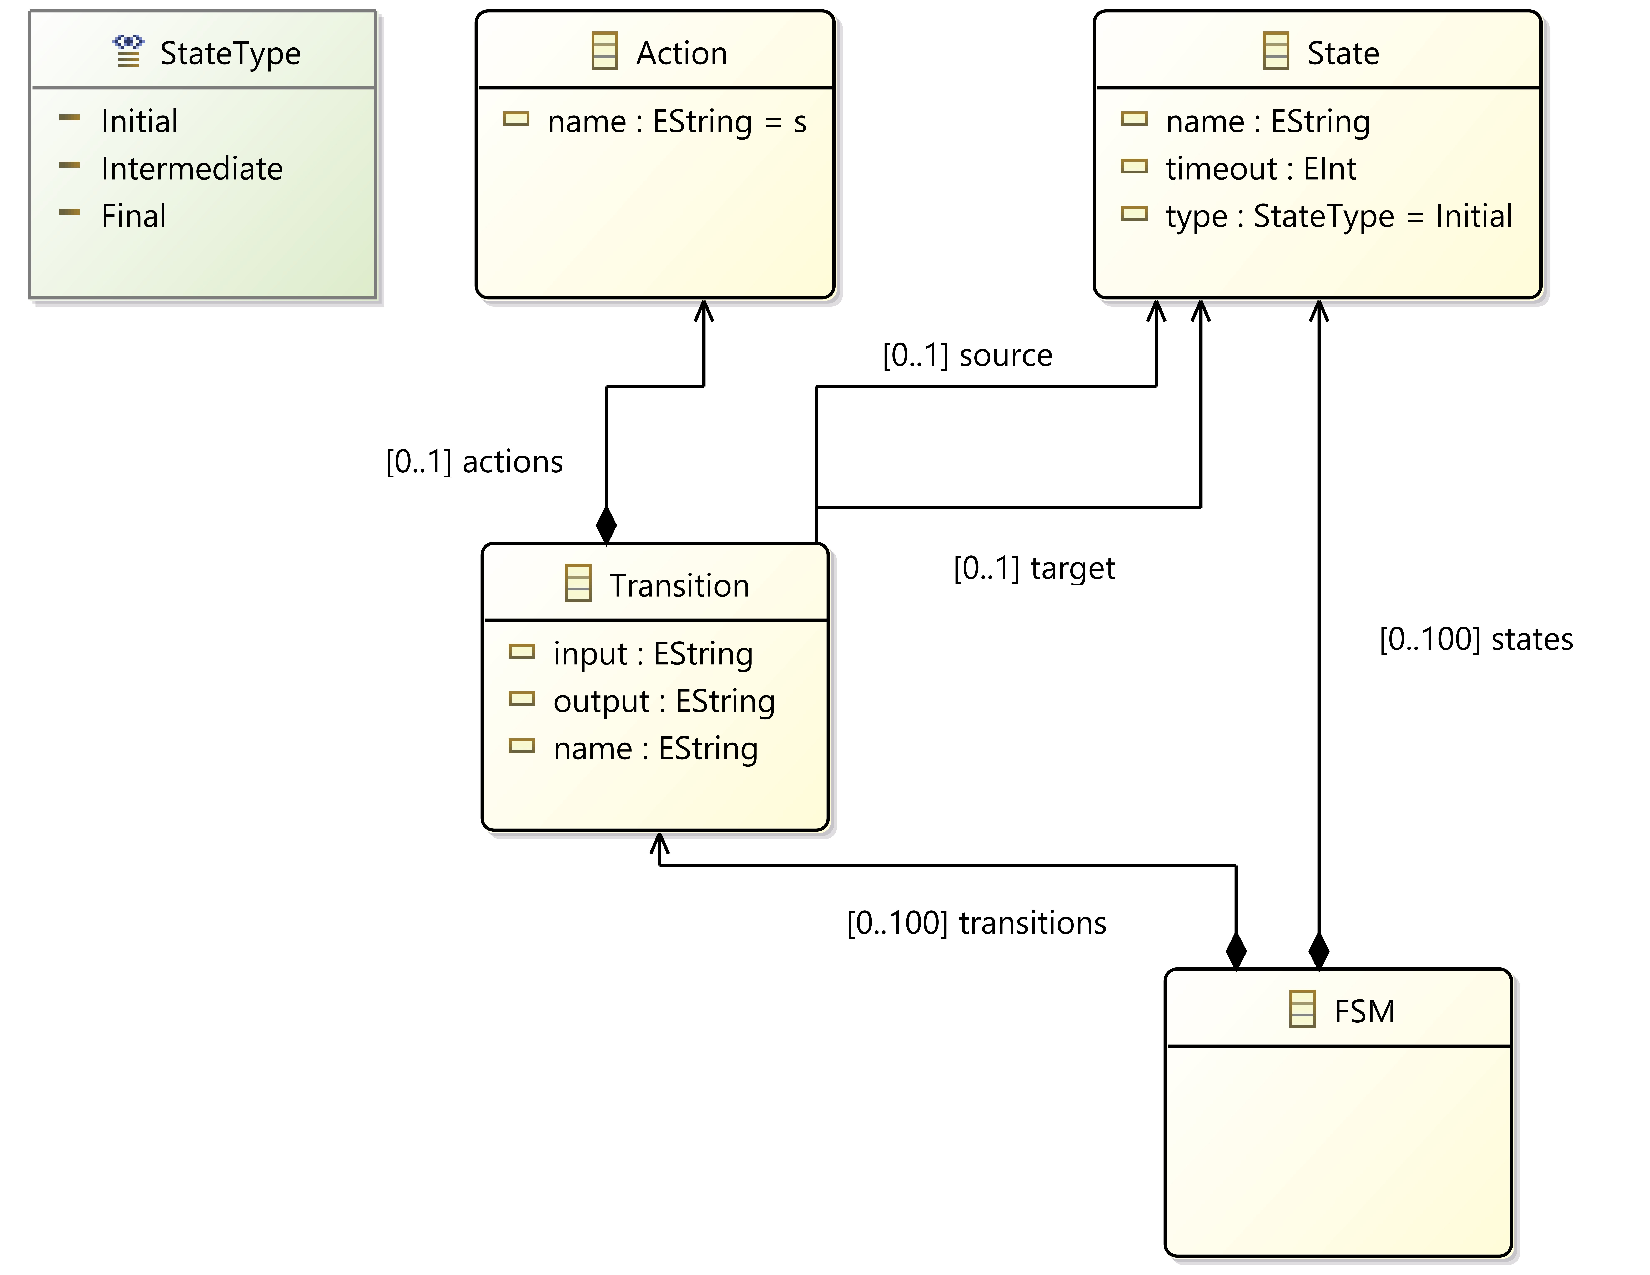
\includegraphics[width=8 cm]{Figures/ecorediagram.pdf}
    \caption{The ecore diagram of a FSM.\label{fig:ecoremodel}}
\end{figure}

\begin{figure}[H]
    \centering
    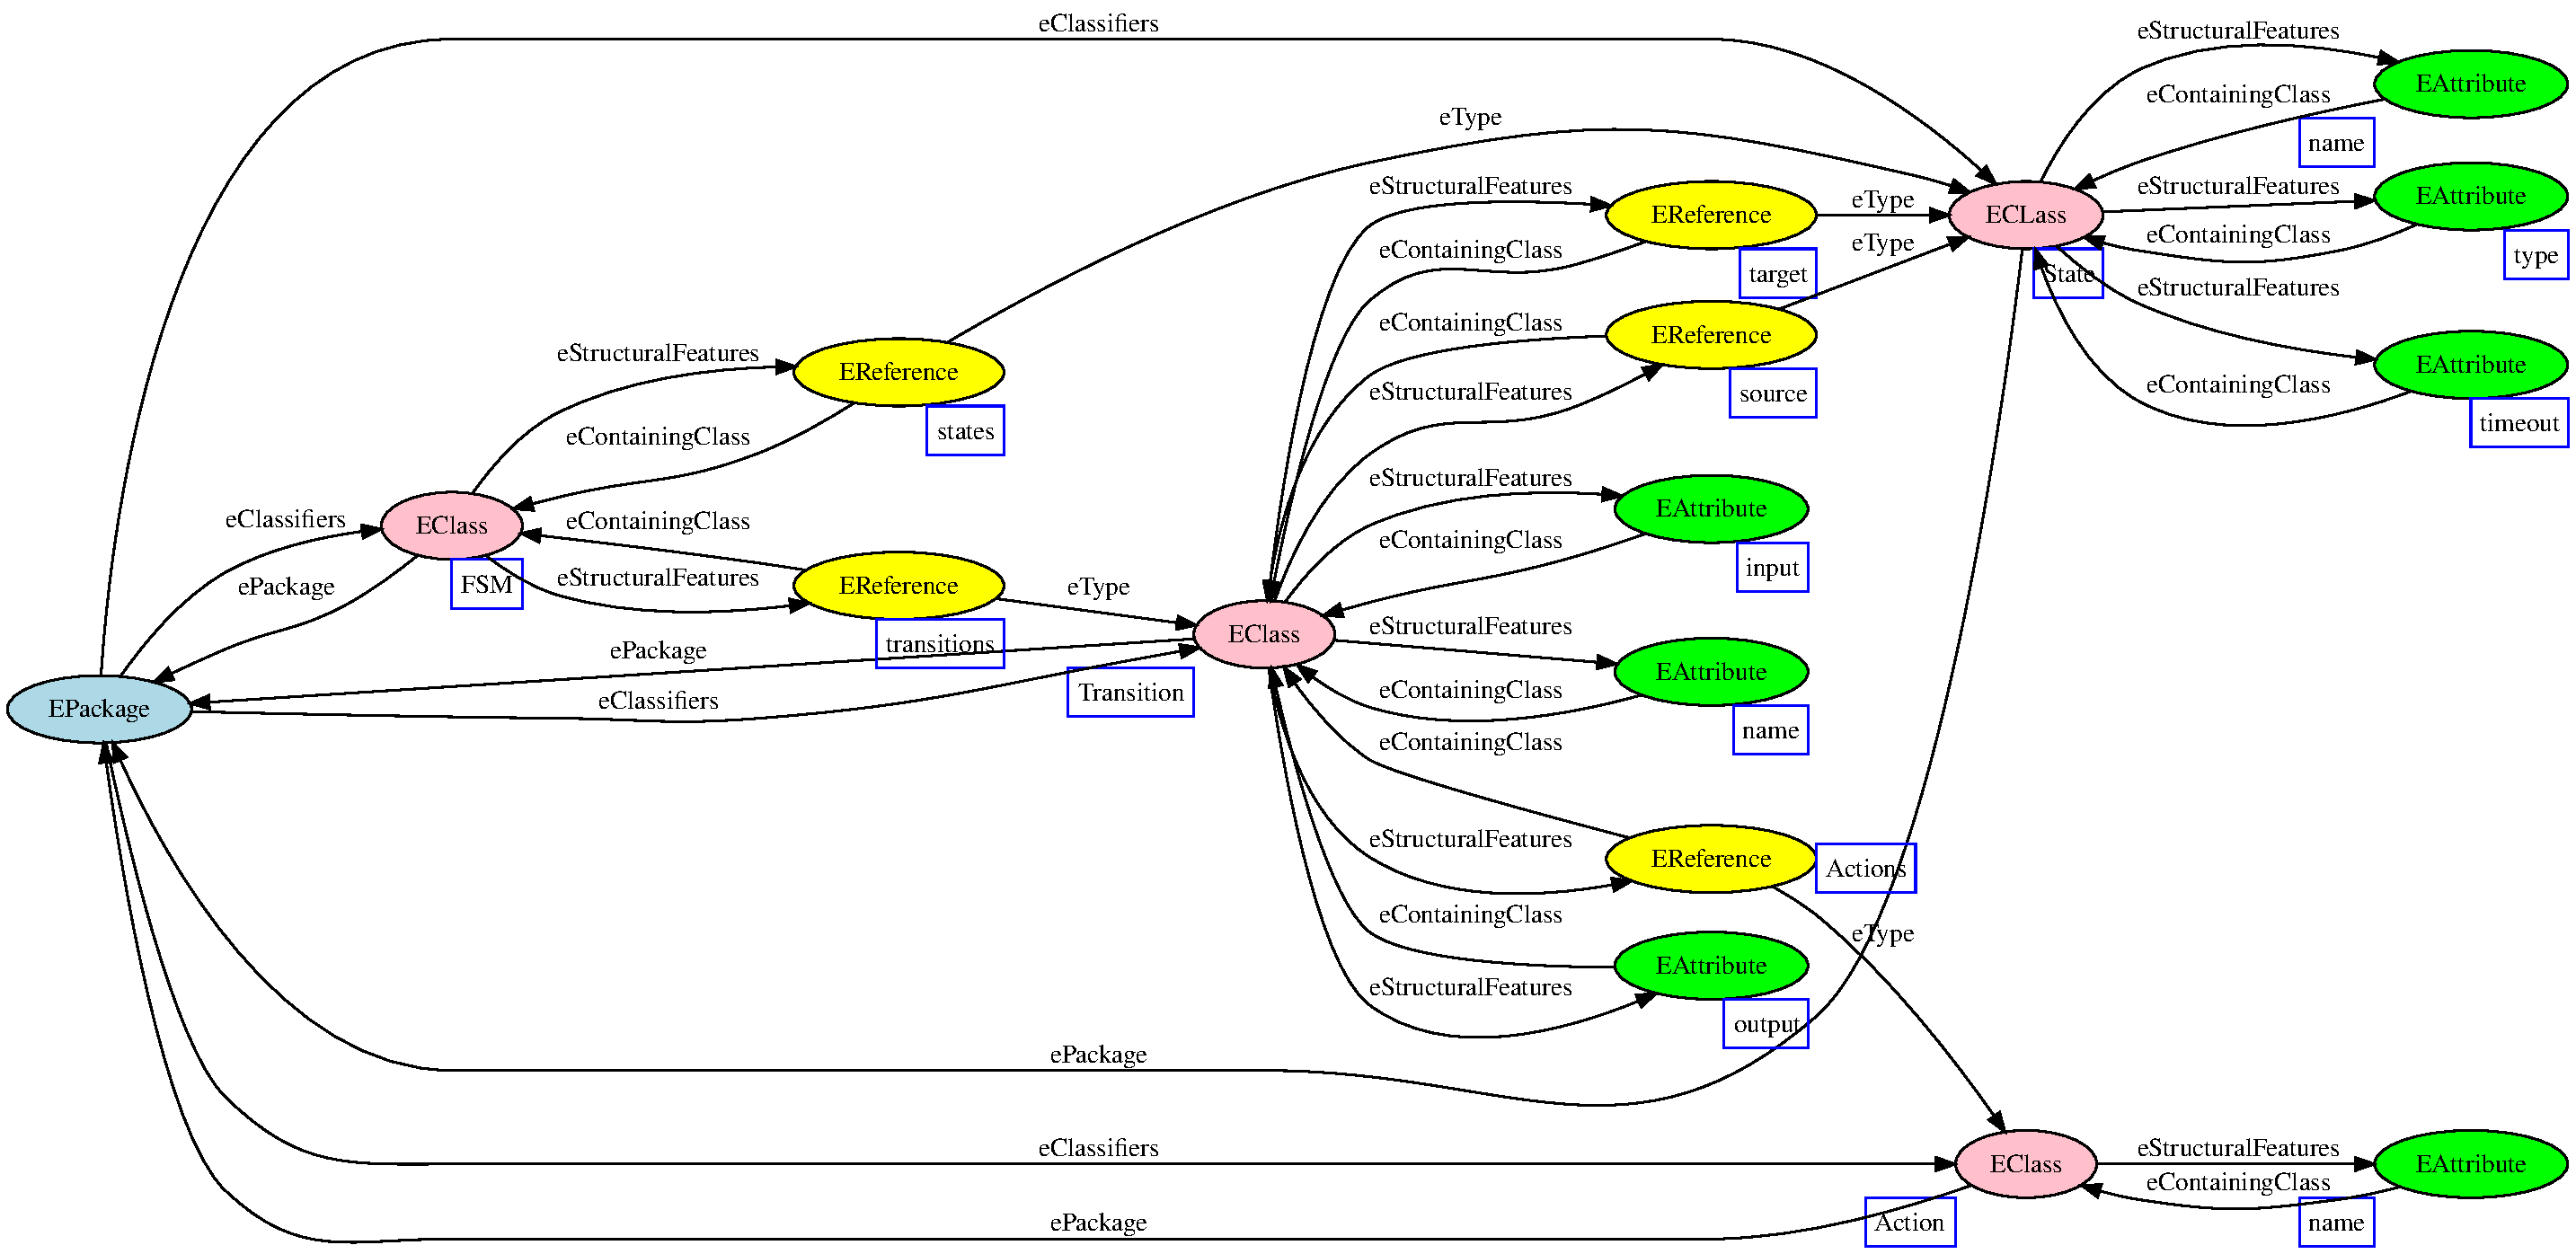
\includegraphics[width=\textwidth]{Figures/ecoregraph.pdf}
    \caption{The corresponding graph of the metamodel in Figure~\ref{fig:ecoremodel}.\label{fig:ecoregraph}}
\end{figure}

\begin{figure}[H]
    \centering
    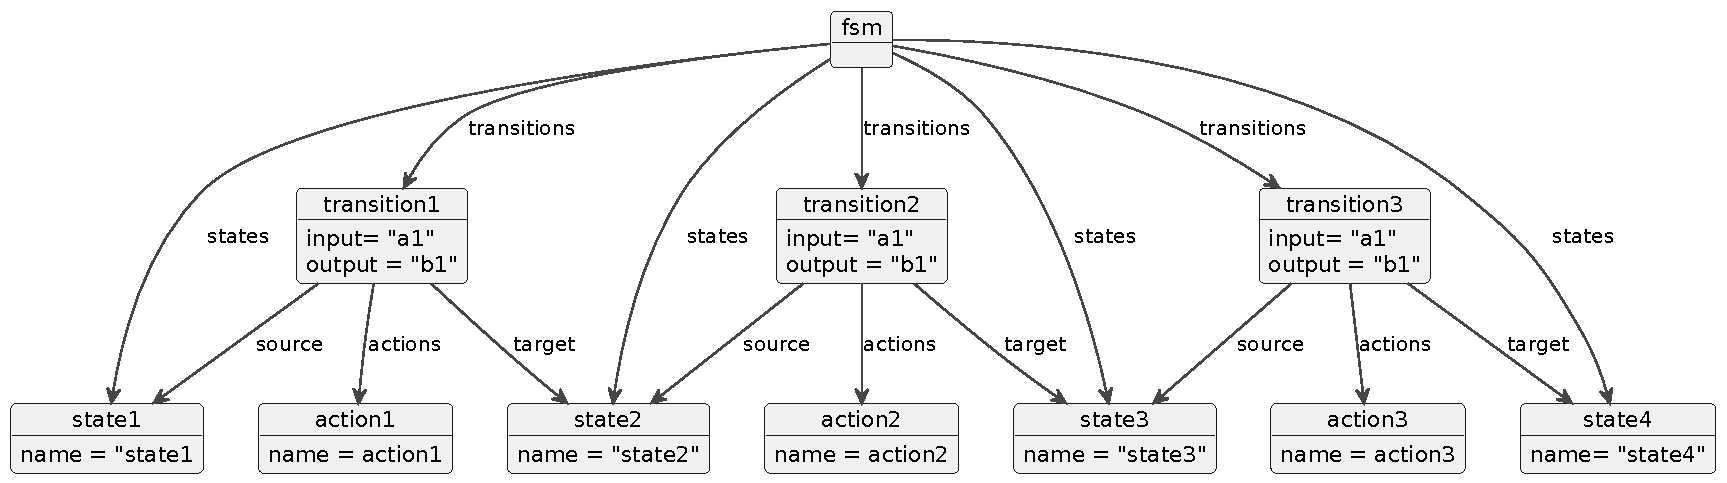
\includegraphics[width=\textwidth]{Figures/object diagram.pdf}
    \caption{An instance model of the FSM in Figure~\ref{fig:ecoremodel}.\label{fig:objectdiagram}}
\end{figure}

\begin{figure}[H]
    \centering
    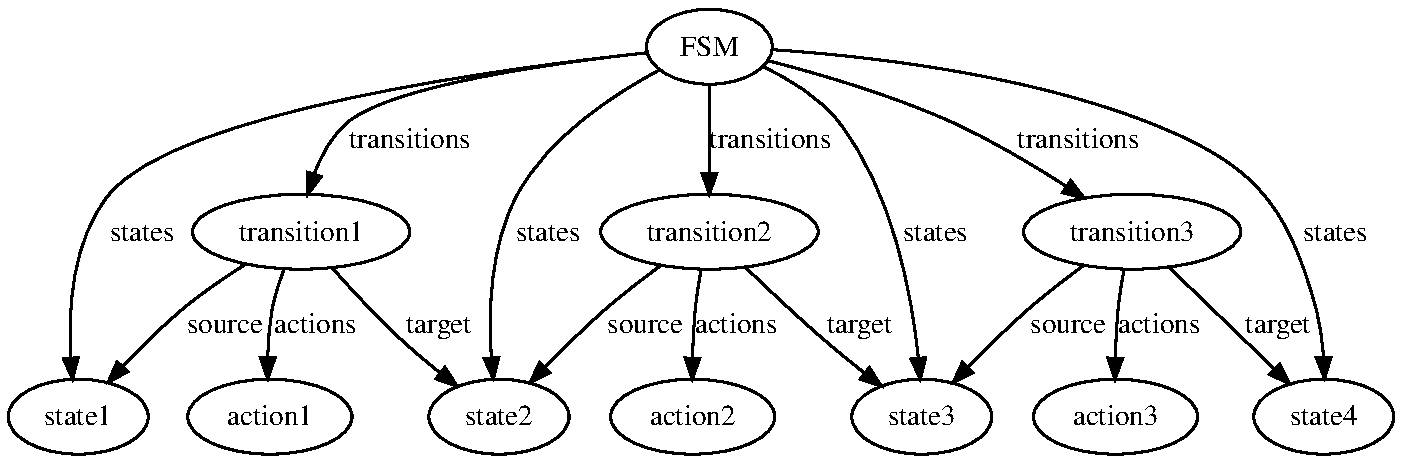
\includegraphics[width=10 cm]{Figures/object graph.pdf}
    \caption{A graph corresponding to the instance model in Figure~\ref{fig:objectdiagram}.\label{fig:objectgraph}}
\end{figure}


\section{Encoding Process} \label{sec:EncodingProcess}
The architecture of our proposed encoding of models is illustrated in Figure~\ref{fig:Structure}. It consists of three main technical spaces: model engineering, data gathering, and graph presentation technical spaces. In the first phase, the input models and associated metamodel are loaded into the PyEcore library. This enables navigation of the model and extraction of raw data by interfacing with the model elements.

In the next phase, the MoEGL configuration is loaded to check for necessary adaptations. The MoEGL configuration, written by the user, conforms to the configuration meta-model proposed in Figure~\ref{fig:Structure}. It is described in more detail in the next section. First, all the model elements are extracted and serialized to separate CSV files stored locally. With the MoEGL configuration, the desired elements are extracted from the files. The data are organized into three levels including node data, edge data, and attribute type data. For example, the organization of the node and edge data for the model in Figure~\ref{fig:ecoremodel} would be as follows: The node data contains one EPackage file with the EPackage data, four EClass files with the EClass object data, five EReference files with the EReference object data, and seven EAttribute files with the EAttribute objects data. The edge data files contain EPackage--EClass edges, EClass--EPackage edges, EClass--EReference--EClass edges, EClass--EReference edges, and so on.

Finally, the data extracted from the organized files are transformed into an in-memory representation according to the user needs specified in the MoEGL configuration. We provide two output graph formats, including the NetworkX and Heterogeneous PyTorch Geometric (HPyG) graphs. MoEGL is described in more detail in the following section.

Existing works in the literature employ NetworkX for representing models as homogeneous graphs. We add support for mapping models to heterogeneous graphs. These graph types are more precisely aligned with the model structures, by supporting node types associated with sets of attributes, thus allowing object attributes to be directly represented.

\begin{figure}[H]
    \centering
    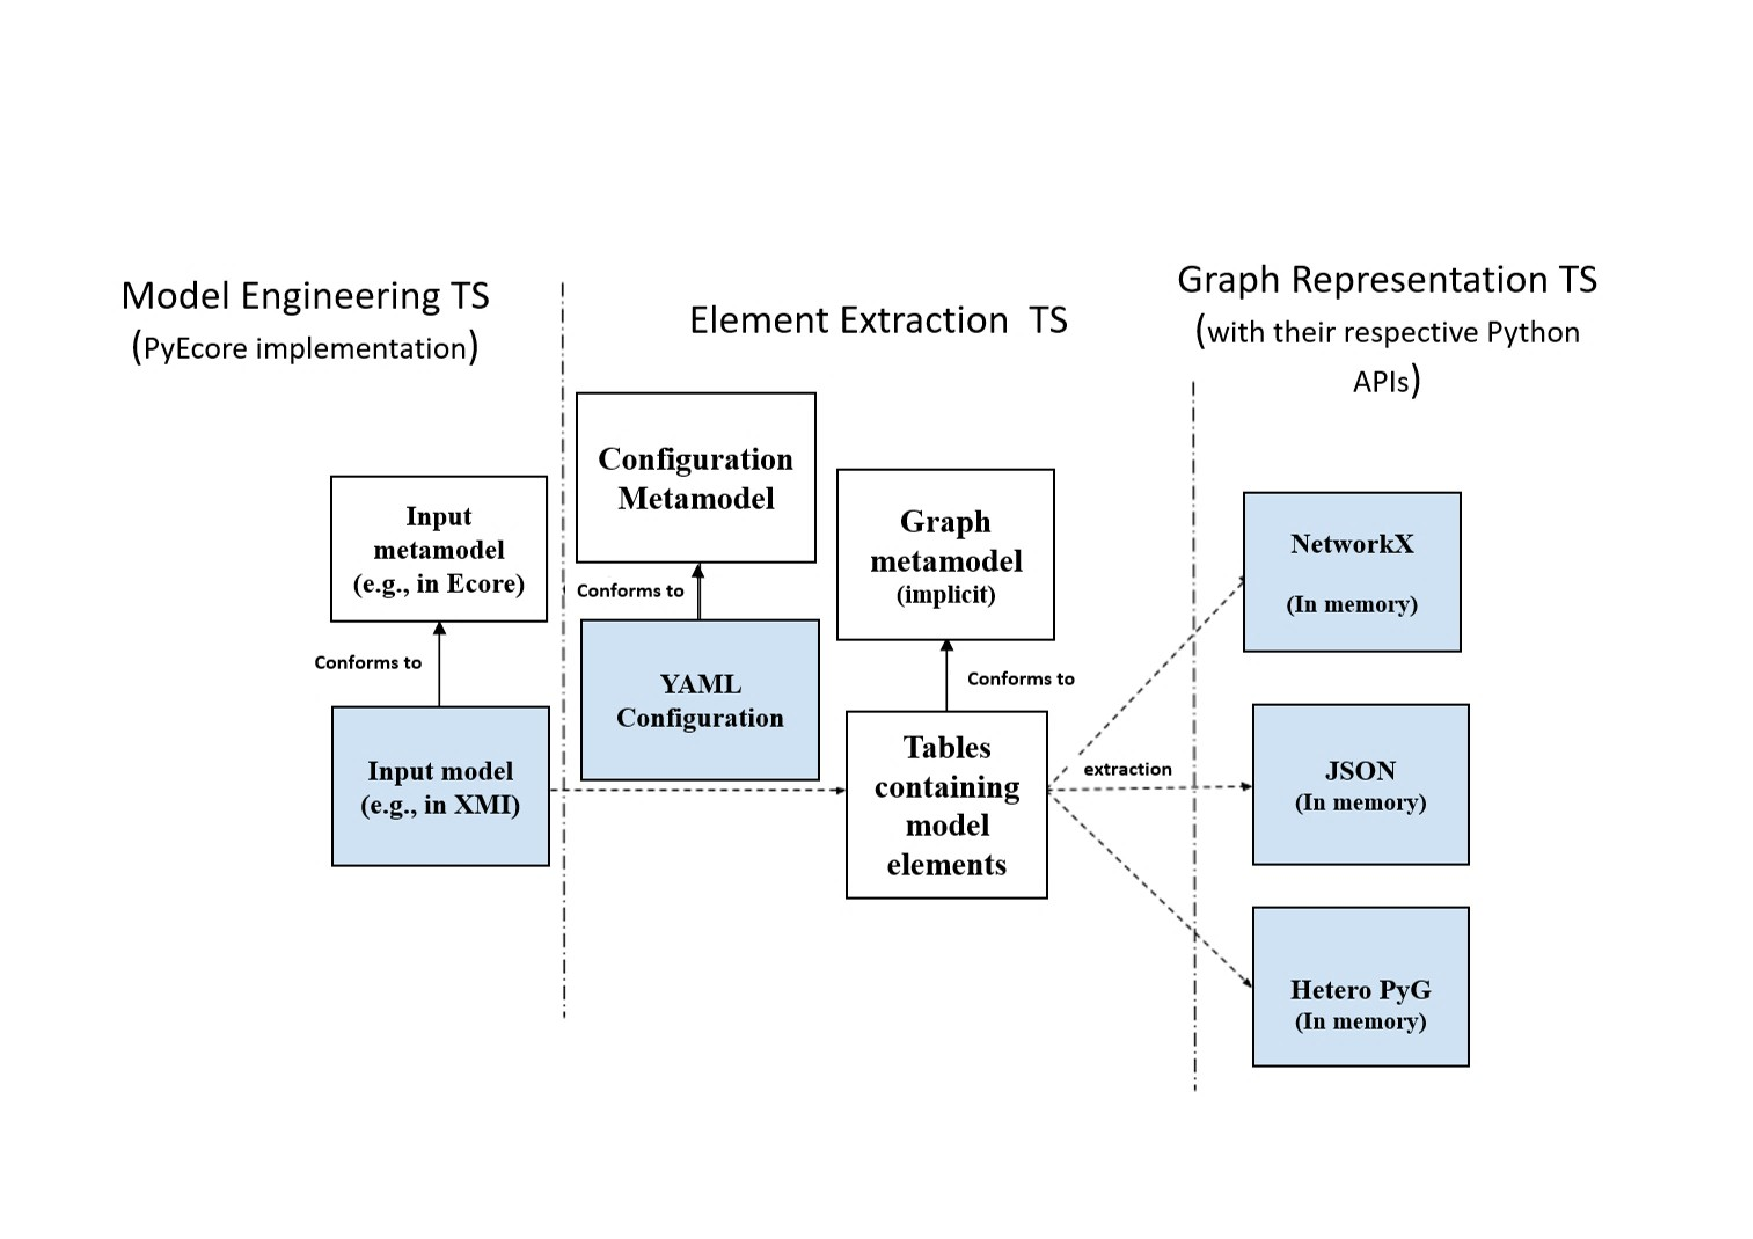
\includegraphics[width=10 cm, trim = 2cm 3cm 2cm 2cm]{Figures/structure.pdf}
    \caption{The architecture of the proposed process.\label{fig:Structure}}
\end{figure}

\subsection{Heterogeneous Graph Construction} \label{Heterogeneous graph}
A heterogeneous graph is a general graph model that can represent multi-typed entities and relations. As defined by Sun et al.~\cite{sun2012mining}, a heterogeneous graph G is represented as \(G = \{V, E, \phi, \psi\} \) where V is the set of nodes, E is the set of edges, \(\phi(v)\) assigns a type to each node $v$, and \(\psi(e)\) assigns a type to each edge $e$. More specifically, \(T_v = \{\phi(v): \forall v \epsilon V\}\) contains the distinct node types defined in the graph schema, and \(T_e = \{\psi(e): \forall e \epsilon E\}\) contains the distinct edge types. This typing of both nodes and edges allows a heterogeneous graph to represent diverse semantic entities and their interconnectivity in a structured manner. The graph degenerates into a regular homogeneous graph when \( \mid T_v \mid = \mid T_e \mid = 1 \), meaning there is only one node and one edge type.

Here, we undertake an in-depth examination of the encoding technique applied to various input models, such as metamodels and instance models, comparing this encoding approach to representations utilized in prior work. Considering the metamodel of the FSM in Figure~\ref{fig:ecoremodel}, it contains 1 node of type ``EPackage'', 4 nodes of type ``EClass'', 5 nodes of type ``EReference'', and 7 nodes of type ``EAttributes''. As illustrated in Figure~\ref{fig:ecoregraph}, nodes sharing an equivalent color within the graph possess an identical type, attribute set, and relationship configuration. When metamodels are encoded as graphs, node attributes serve to represent the properties belonging to each object (referred to as metadata). For instance, an ``EClass'' node might contain an ``abstract'' attribute, whereas an ``EReference'' node could outline attributes such as ``lowerBound'', ``upperBound'', ``ordered'', ``unique'', ``required'', ``changeable'', and ``volatile''. These properties aid tasks involving the architectural structure of metamodels, including but not limited to model generation, completion, and ML applications.

Considering the instance model depicted in Figure~\ref{fig:objectdiagram}, it contains four types of nodes (fsm, transition, state, and action) and five types of edges (transitions, states, source, target, and actions). Additionally, the individual nodes themselves carry substantial attribute information (e.g. name, input, output, type, and timeout). Furthermore, the various relationships between the nodes convey richer semantic information. Due to the diversity of node and edge types present, a homogeneous graph alone is unable to represent all facets of the information within the model. When handling nodes and relations with different semantics in such models, graphs originally proposed using homogeneous structures may encounter notable obstacles. In previous work, node types in homogeneous graphs have been managed by defining a ``type'' attribute for each node. HGNNs are able to learn on attributes with different types stored for each node type, effectively handling the inherent complexity of heterogeneous graphs. This complexity arises because, unlike homogeneous graphs where all nodes share the same set of attributes, heterogeneous graphs contain multiple types of nodes and edges, each with unique attributes and relationships. HGNNs address this challenge by utilizing specialized mechanisms to process and integrate these diverse attributes and structural information. They employ tailored aggregation functions to capture the semantic and structural information unique to each node type, ensuring that the rich semantic and structural diversity of heterogeneous graphs is preserved and leveraged effectively for various applications.

\section{MoEGL: Encoding Configuration DSL} \label{Sec:encodingconfigurationDSL}
We propose MoEGL, a DSL to flexibly encode domain models as graphs tailored to users' needs. We defined a list of requirements for MoEGL, that we used to drive its design. We list them here, and in Section~\ref{Sec:Experiments} we will show that by satisfying such requirements, MoEGL performs well w.r.t. our research questions.

\begin{itemize}
    \item MoEGL syntax must be simple, clear, and unambiguous to avoid any misinterpretations. Static checks on model elements are also important. This includes ensuring the uniqueness of class and feature names within the same package.
    \item The language must be familiar and intuitive for users. Using YAML, a widely known data serialization format, can help with this.
    \item There also needs to be a strategy to prevent naming collisions between generic encoding properties and meta-model elements
    \item All EMF metamodels (including cyclic ones) have a hierarchical containment structure. We want to organize MoEGL based on this structure, which is already familiar to EMF practitioners. This way we can also statically assess consistency with the EMF metamodel, and its coverage. As a consequence of this choice our handling of cycles is limited, as we can copy them or remove them, but we can not create new cycles. This is however sufficient for our needs, since the encoding process does not generally modify the structural properties of the graph.
    \item It is crucial to support different output formats suitable for diverse user needs.
    \item The language must allow access to all meta-model elements and features via YAML sections.
    \item Crucially, MoEGL needs options to flexibly adapt the meta-model structure as required. For example, renaming model elements or encoding attribute values. This level of customization is key to meeting varied user requirements.
\end{itemize}
Overall, satisfying these design goals can result in a DSL that empowers domain experts to concisely yet precisely define their models and map them to graphs as per their specific application needs. MoEGL aims to strike an ideal balance of usability and expressiveness.

We implement our language as a schema defined within the YAML format. YAML~\cite{ben2009yaml} serves as a data serialization framework. It incorporates various segments such as structural details and raw informational payloads. YAML presents a relatively straightforward usage while maintaining compatibility with many common programming languages like Python. The relationships, characteristics, and organization of MoEGL are visualized conceptually through the class diagram presented within Figure~\ref{fig:DSL_Diagram}. This diagram outlines the primary abstractions, their attributes, and the connections between these abstractions that underlie the structure and functionality of the language that has been constructed to serve the needs of the targeted domain. The structure of possible sections and values in YAML is shown in Listing~\ref{code:Yaml}. All the code implementations of the proposed DSL are available on GitHub at \url{https://github.com/Z-Rajaei/MoEGL}.

\begin{figure}[H]
    \centering
    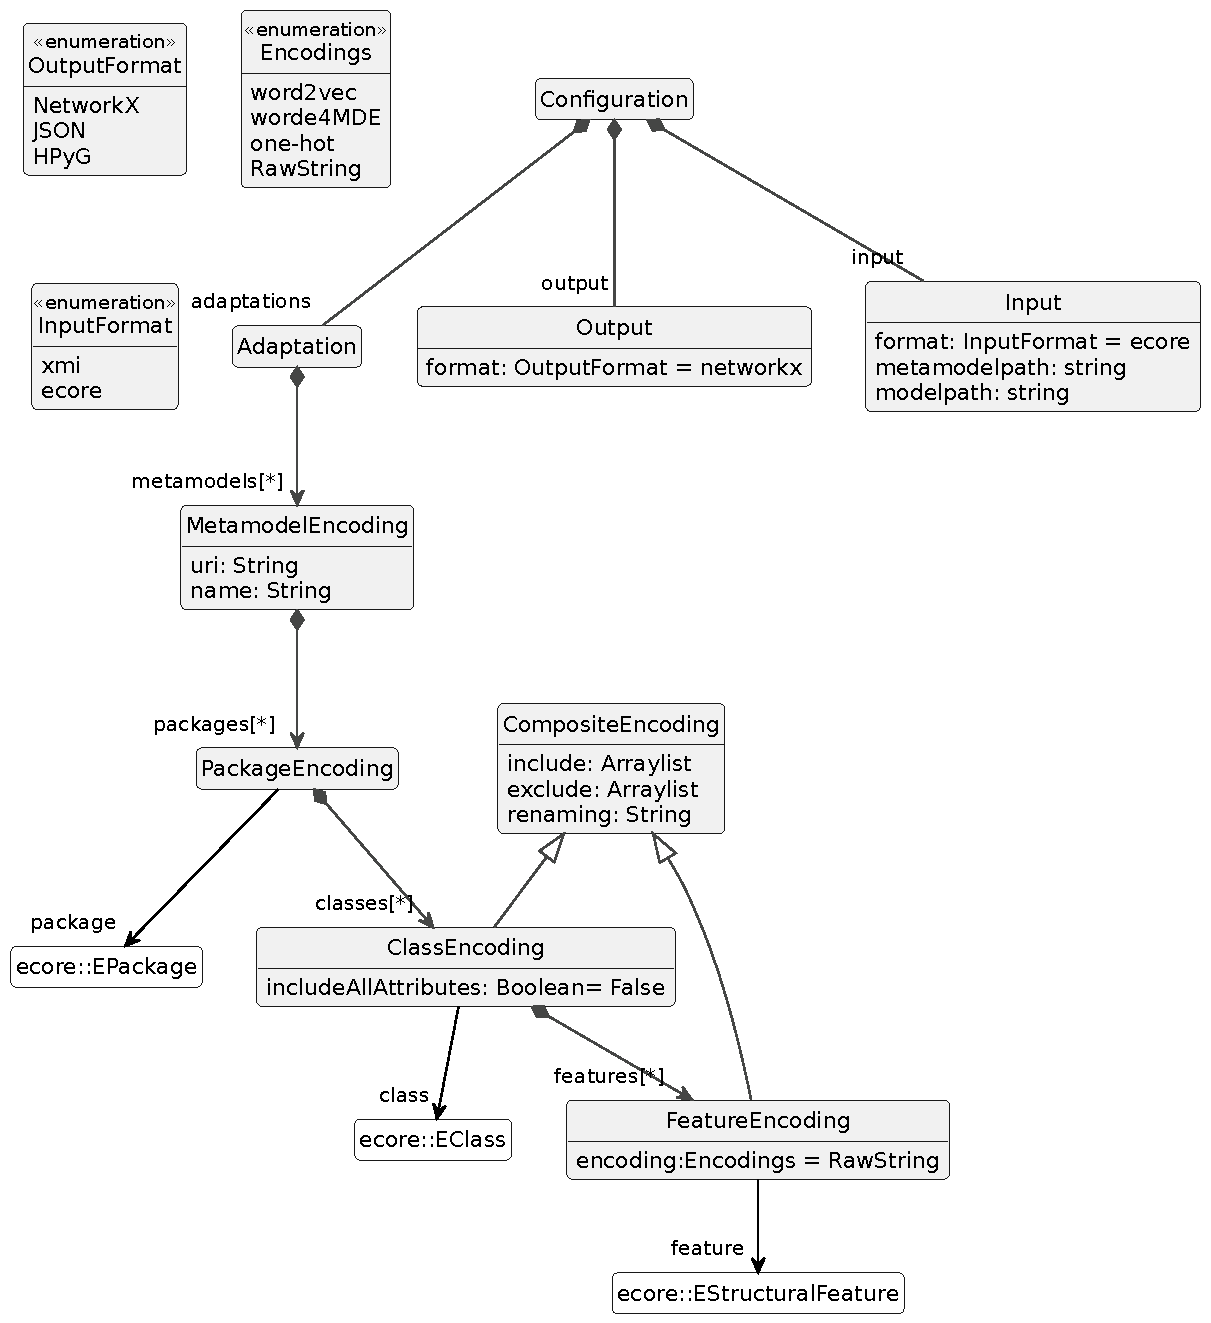
\includegraphics[width=12 cm]{Figures/DSL_diagram.pdf}
    \caption{The class diagram of MoEGL.\label{fig:DSL_Diagram}}
\end{figure}


\begin{program_}[H]
\footnotesize
\begin{verbatim}
inputmodels:
  -format: "ecore/xmi"
  -metamodelpath: "Path_to_metamodel"
  -modelspath: "Path_to_models"
output: "NetworkX/HPyG"
adaptations:
  -metamodels:
    -packages:
      -"ecore_name":
        -uri:
          -http://www.eclipse.org
          /emf/2002/Ecore:
          -classes:
          -include:
            ["name_of_included_
            Eclass_elements"]
          -exclude:
            ["name_of_included_
            Eclass_elements"]
          -includeAllAttributes: True/False
          -"Name_of_desired_EClass":
            -include:
            ["name_of_included_features"]
            -exclude:
            ["name_of_excluded_features"]
            -renaming:
            "new_name_for_EClass"
            -features:
              -"Name_of_desired_feature":
                -renaming:
                "new_name_for_EClass"
                -encoding:
                "RawString/word2vec
                /worde4MDE/one-hot"
\end{verbatim}
\caption{The structure of a YAML file.}
\label{code:Yaml}
\end{program_}


The MoEGL configuration contains three principal sections that guide how the models are adapted, what data is taken in, and how the results are generated. This includes ``adaptation'', ``input'', and ``output''. The ``adaptations'' section allows for customizing how the elements from the metamodel are encoded as nodes and edges in the graph. This preprocessing is necessary to transform the models into a format that is suitable for various ML tasks. Each adaptation incorporates one or more ``MetamodelEncoding'' components empowering the user to get to the intended metamodel through the ``name'' and ``URI'' addresses of its package. Under each ``PackageEncoding'' are ``Class Encoding'' components that allow the user to selectively include or exclude which model element classes will be represented as nodes in the final encoded graph. Individual classes can then be further configured via their name, where the features of each class can be selectively included or excluded at the attribute and reference level. The user can also specify whether all class attributes participate in encoding using ``includeAllAttributes''. We do not need to provide OCL constraints, since we define a policy to unambiguously handle every combination of these operators. In our policy, attribute exclusions have the highest priority, followed by attribute inclusions. For instance, if ``includeAllAttributes'' is followed by an ``exclude'', the DSL will include all the attributes that are not explicitly excluded.

The capabilities of the MoEGL configuration allow users to selectively determine which model aspects are included or excluded in/from the final representation. Individual characteristics can be included or excluded from the final encoded graph structure by utilizing their given names or labels in conjunction with the ``include'' and ``exclude'' directives. Features can be included or excluded by name using ``include'' and ``exclude''. A feature can be an attribute or a reference. If the excluded feature is a containment reference, the program simply removes the reference and not the target class. Therefore, if we also need to remove the target, it should be excluded explicitly by the ``exclude'' option in the class section. When a containment reference is excluded, the program removes the reference because it represents the relationship or linkage between elements rather than the elements themselves. The target class, being a separate entity, is not automatically removed to preserve the integrity of other potential references or usages within the model. If the target class were to be removed automatically, it could inadvertently affect other parts of the model that rely on it. Therefore, to ensure precise and controlled modifications, the user must explicitly exclude the target class in the class section. This approach maintains the model's consistency and prevents unintentional deletions that could disrupt the overall structure and functionality of the model.

Each class offers attribute configuration. Similarly, the user can access classes as shown in the diagram. Renaming modifies element names for tasks involving the comparison of metamodels with identically named but distinct attributes. For instance, the user can specify in the DSL that a ``surname'' attribute should be renamed to ``lastname'', so that it will share the same encoding of another ``lastname'' attribute in the metamodel.
The feature encoding section specifies how the values of attributes and references should be represented, such as raw strings or using vector representations obtained via techniques like word2vec. Further explanation is provided regarding these encoding representations and techniques later on. The ``input'' meta-schema specifies the data format of source models, as the declarative language is designed to encode models defined in both Ecore and XMI formats. Relevant file paths must also be set for both the metamodel and models. The desired output graph format such as NetworkX or HPyG is then configured within the output section settings. Proper configuration of input data retrieval and desired output formatting is crucial for effectively transforming models into machine-readable graph structures while preserving original semantic meaning.

The declarative schema language therefore provides access and manipulation capabilities applicable to full metamodels, individual model classes, and even single attributes or references. The second major processing stage depicted in Figure~\ref{fig:Structure} relies on these pre-encoding adaptations and configurations by way of a specified Python method to selectively check and include only relevant model aspects.

\subsection{Encoding Attribute Values}\label{sec:avalues}
By default, we use raw values for encoding numerical attribute values. However, for string values, the user can choose an encoding based on her models and ML goals. String values can also be encoded with embedding techniques like word2vec or WordE4MDE. word2vec maps each unique string to a dense numerical vector of fixed size, capturing semantic meaning. Similar strings have close vectors, allowing semantics rather than surface form to relate strings. These embeddings support analyzing string relationships based on content. word2vec thus has the potential to support tasks involving predictive analysis of attribute values.

Word4MDE~\cite{lopez2023word} is a variant of word2vec tailored to the domain of modeling languages and is particularly well-suited for the above tasks as its word embeddings are trained on a large corpus of actual element names and labels from models. This specialized training enables Word4MDE to capture important linguistic patterns and semantic relationships that are specific to modeling domain terminology. The embeddings it generates therefore provide a more accurate representation of semantic similarity as it pertains to the names and labels used in modeling languages.

Categorical attributes that describe element or relationship types can be encoded using one-hot encoding. This involves mapping each unique category to a binary vector, with a 1 in the index of the present category and 0s elsewhere. One-hot encoding transforms categorical data into a numerical format while retaining the distinction between different categories. This encoding supports various predictive tasks involving element types.

Given our specific implementation which first extracts and saves all model components, we traverse the models during the construction of their corresponding graphs, extracting all words present in the input models. Based on this list of words, we construct and encode the word2vec model. This approach ensures that the word2vec model, trained on the extracted data, provides meaningful embeddings by capturing the contextual relationships present in the original models.

We were also able to implement one-hot encoding for the same reason, as we have the list of possible values for each attribute. This method also provides an additional benefit, allowing the user to parse and run the models once, performing any desired type of encoding or customization on the models multiple times.
Figure~\ref{fig:fusion} illustrates the described process. The structure and attributes of each model are derived and extracted from the models. The final graph contains both the relational framework of the associations between models as well as the numerically encoded attribute values appointed to each individual node. Once completed, the graphs are then input as data into a GNN system. The neural network will utilize the combined structural and characteristic information from the graph to discern relationships and perform some analytical task, such as classification or prediction, based on the features and connections within the graphical portrayal of the original collection of models.

\begin{figure}[H]
    \centering
    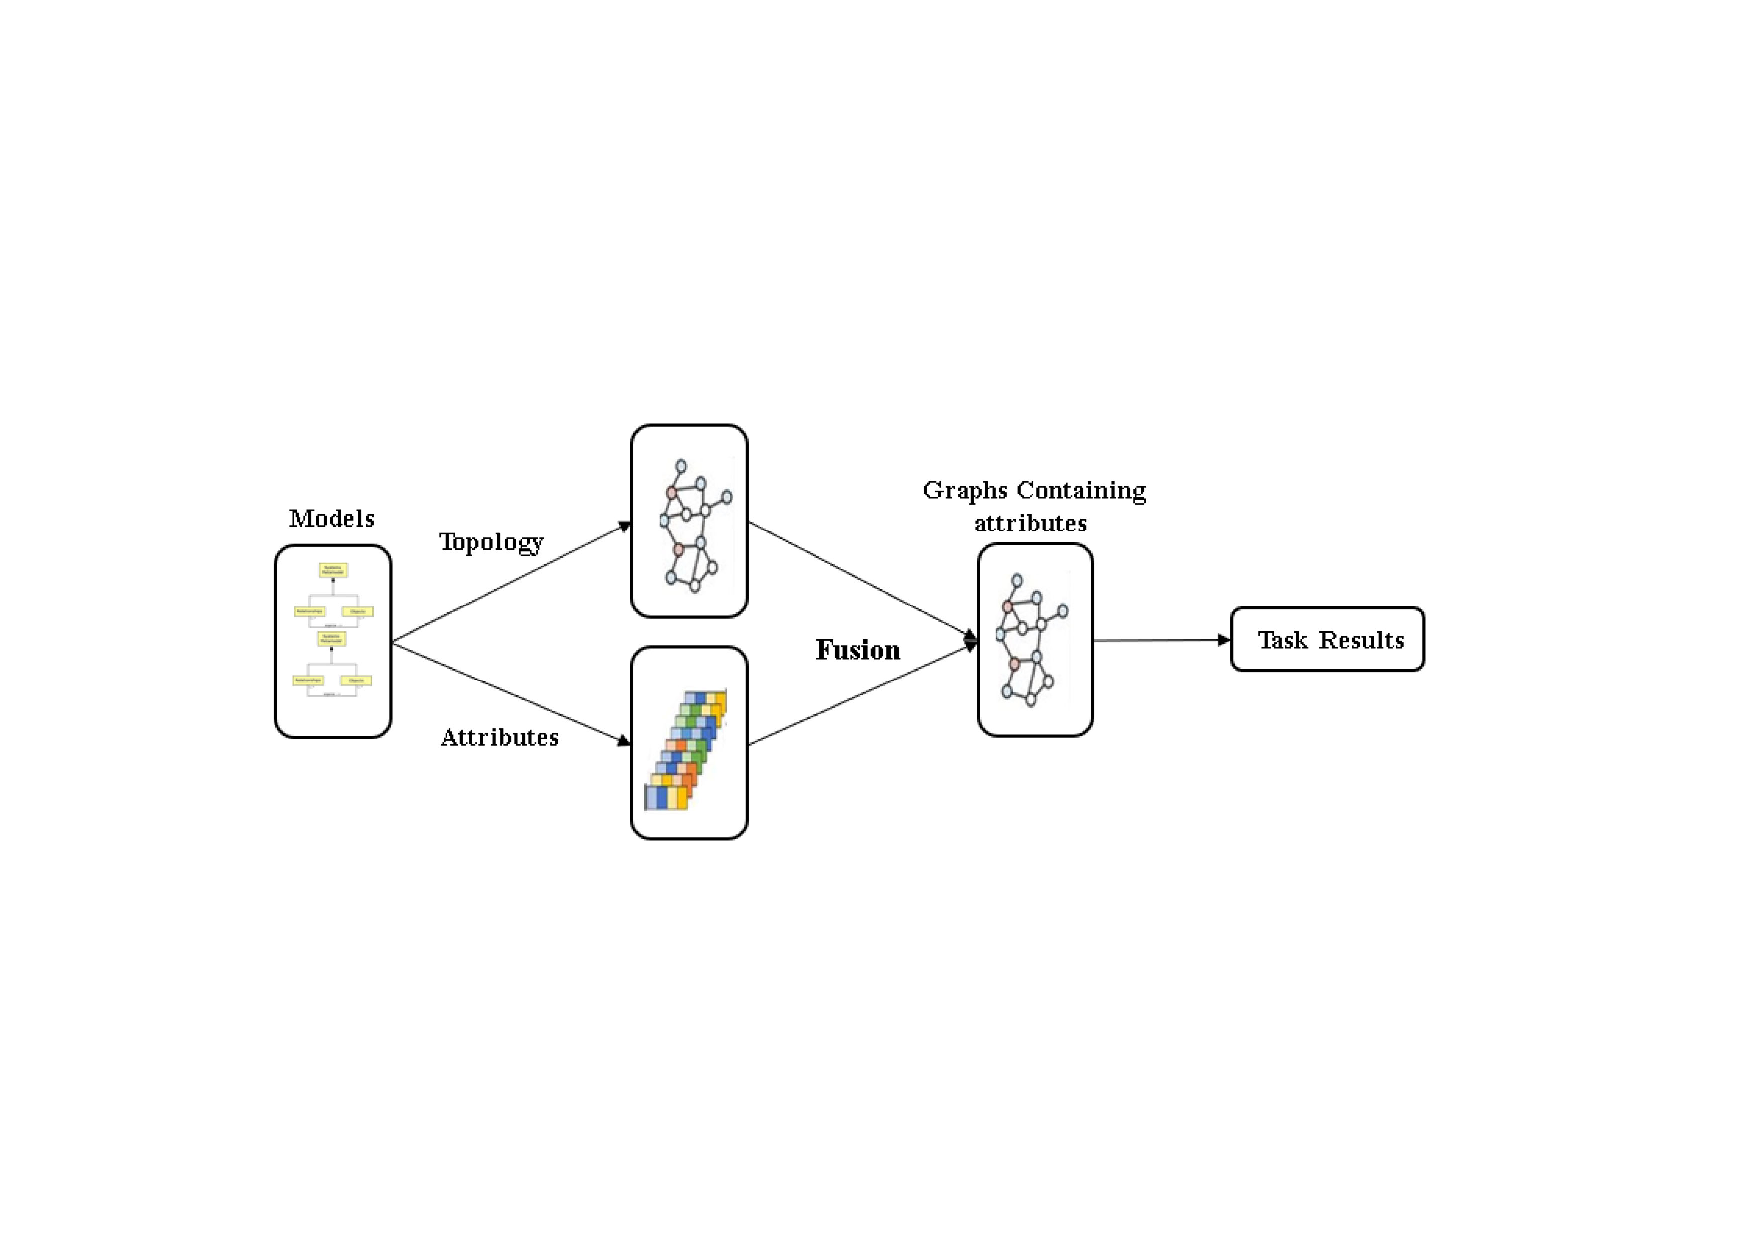
\includegraphics[width=10 cm, trim = 5cm 6cm 6cm 6cm]{Figures/Fusion.pdf}
    \caption{Diagram of extracting model structure and attributes for final graph.\label{fig:fusion}}
\end{figure}

\subsection{Technical Implementation of MoEGL}
In this section, we describe the detailed implementation process of MoEGL, highlighting the key steps involved in transforming models into graph structures suitable for Graph Neural Networks (GNNs). Our approach follows a structured process that includes model traversal, application of filtering rules, encoding of node and edge features, and the construction of both homogeneous and heterogeneous graphs.

\textbf{1. Model Traversal and Element Extraction.}
The first step in our pipeline is the traversal of the input models, which can be provided in either ecore or xmi formats. Depending on the format, we load and traverse the models to extract key elements, such as nodes and edges. During this traversal, the model elements are systematically processed, and for each element, we capture its attributes and references. This hierarchical traversal ensures that all relevant model elements are visited and prepared for inclusion in the resulting graph structure.

\textbf{2. Node and Edge Creation.}
As the model elements are traversed, we generate nodes and edges corresponding to each element and its relationships. Nodes are created for each class instance in the model, with their attributes stored for later use in encoding. Similarly, edges are generated to represent the relationships between different nodes, reflecting the references in the original model. This process ensures that the structure of the input model is accurately preserved in the graph, maintaining the hierarchical and referential integrity of the data.

\textbf{3. Application of Filtering Rules.}
To provide flexibility in model-to-graph transformation, we apply user-defined filters from the configuration file during the graph construction process. These filters allow users to specify which classes and attributes should be included or excluded from the final graph. The filtering is performed in two stages:

Node Filtering: Nodes are included or excluded based on the classes they represent, as defined in the filters. Users can also specify whether all or only certain attributes of a class should be included.
Edge Filtering: Edges connecting nodes are filtered similarly, ensuring that only the relationships of interest are represented in the final graph.
This customizable filtering mechanism allows users to tailor the graph representation to their specific needs, reducing complexity and focusing on the most relevant parts of the model.

\textbf{4. Feature Encoding.}
Once the nodes and edges are filtered, we proceed with encoding their attributes into formats suitable for machine learning. Depending on the user's configuration, various encoding techniques are applied, including:

One-Hot Encoding: Categorical attributes are encoded using one-hot vectors, which is useful for representing discrete variables.
Word2Vec Encoding: For textual attributes, we employ Word2Vec embeddings to capture semantic relationships between words in the model. This provides a dense, continuous representation of text data.
Custom Embeddings (worde4mde): For domain-specific terms in the model, we use a custom embedding technique that maps specific terms to pre-trained embeddings, ensuring that the domain knowledge is accurately reflected in the graph's features.
These encoding techniques transform the raw attributes of the nodes and edges into feature vectors that can be consumed by GNNs.

\textbf{5. Graph Construction.}
After encoding the node and edge features, the graph is constructed. We support two types of graph structures:

Homogeneous Graphs: In this configuration, all nodes and edges are of the same type, which is useful for simpler models where there is no need to distinguish between different types of entities.
Heterogeneous Graphs: For more complex models, we construct heterogeneous graphs, where nodes and edges can have multiple types. This allows us to preserve the distinct types of entities and relationships present in the model. The heterogeneous graphs are constructed using libraries such as PyTorch Geometric, which provides efficient handling of different node and edge types for machine learning tasks.

\textbf{6. Output Formats.}
Finally, the constructed graphs can be output in various formats, depending on the user's requirements. We support both NetworkX (for homogeneous graphs) and PyTorch Geometric (for heterogeneous graphs). This flexibility allows the encoded graphs to be used directly in different GNN frameworks, enabling seamless integration with downstream machine learning pipelines.


\subsection{Applying MoEGL to the Running Case}\label{sec:applying}
Assume that a user is working with a dataset containing thousands of FSM metamodel instances like the one shown in Figure~\ref{fig:objectdiagram}. He wants to map all these models to NetworkX graphs for use in a ML task. However, there are a couple of constraints he wants to apply: 1) Exclude the ``action'' objects from the models, as they are not relevant to the particular learning task he intends. 2) Rename the ``transitions'' edges to simply ``trans'' for consistency.
The user defines the desired constraints and transformations in a YAML configuration file. As shown in Listing~\ref{code:YamlFSM}, only a few lines of code are needed to exclude the action objects and rename the transition edges.
The adjacency matrix of the instance model in Figure~\ref{fig:objectgraph} generated by applying the encoding of Listing~\ref{code:YamlFSM} is shown in Matrix~\ref{mat:matrix}.
Now the user can run the learning tasks, and modify the YAML file to easily experiment with different preprocessing configurations, applying multiple ``passes'' over the dataset to determine the optimal representation for their ML task.

\begin{mat}[H]
\begin{equation}
    \begin{bmatrix}
1 & 1 & 1 & 1 & 1 & 1 & 1 & 1 \\
0 & 0 & 0 & 0 & 1 & 1 & 0 & 0 \\
0 & 0 & 0 & 0 & 0 & 1 & 1 & 0 \\
0 & 0 & 0 & 0 & 0 & 0 & 1 & 1 \\
0 & 0 & 0 & 0 & 0 & 0 & 0 & 0 \\
0 & 0 & 0 & 0 & 0 & 0 & 0 & 0 \\
0 & 0 & 0 & 0 & 0 & 0 & 0 & 0 \\
0 & 0 & 0 & 0 & 0 & 0 & 0 & 0
    \end{bmatrix}
\end{equation}
\caption{Adjacency matrix of the instance model in Figure~\ref{fig:objectgraph} generated with applying the encoding of Listing~\ref{code:YamlFSM}.}
\label{mat:matrix}
\end{mat}


\begin{program_}[H]
\footnotesize
\begin{verbatim}

input:
  format: "xmi"
  metamodelpath: "f:\\fsm.ecore"
  modelspath: "f:\\models"
output:
  format: "NetworkX"
adaptations:
  metamodels:
    packages:
      FiniteStateMachine:
        uri:
          www.fsmmetamodel.com:
            classes:
              exclude: ["Action"]
              fsm:
                features:
                  transitions:
                    renaming: "trans"
\end{verbatim}
\caption{A sample MoEGL program for encoding instance models similar to Figure~\ref{fig:objectdiagram}.}
\label{code:YamlFSM}
\end{program_}

Let us examine in greater detail the process of configuring a more complex MoEGL program to encode the instance model. The user intends to encode the instance model in Figure~\ref{fig:objectdiagram}, which includes various attributes of different types that must be appropriately encoded. The final goal is to train a neural network to automatically generate similar FSM models. Therefore, representing the attribute values accurately will be crucial to the network's ability to learn.

The user has defined a MoEGL configuration to specify how each attribute should be encoded based on its data type. As shown in Listing~\ref{code:YamlFSMattributes}, the MoEGL configuration outlines that string attributes will use word2vec embeddings to vectorize their values. This embedding technique represents words as dense numeric vectors, capturing semantic relationships between terms. Meanwhile, the type attribute that can take on one of just three class labels will employ a one-hot encoding scheme. This involves transforming each class into a binary vector, with a 1 at the index of the class and 0s elsewhere.

Since the nodes of different types have different attributes and references, the graph representing the instance model must support heterogeneous node and edge types. For this purpose, the user has selected the HPyG library, which provides the necessary functionality. With attributes encoded via the prescribed methods, the graph will contain the rich information needed for the neural network to learn patterns. While NetworkX allows nodes and edges to have different attributes, it does not natively support multiple node and edge types as distinct entities. For this purpose, the user has selected the HPyG library, which provides the necessary functionality to handle heterogeneous node and edge types more effectively.


As a demonstration, Figure~\ref{fig:outputFSM} depicts the output graph shape and the matrix for a sample State node within the model. By examining this data, we can observe details like there being one FSM node, four State nodes, three Transition nodes, and three Action nodes in the graph. The various edge types connecting these nodes are also enumerated. Together, the encoded attributes and graph structure capture the key structural and semantic elements of the instance model for the neural network to analyze and potentially generate new similar FSM models.

\begin{program_}[H]
\footnotesize

\begin{verbatim}
input:
  format: "xmi"
  metamodelpath: "f:\\fsm.ecore"
  modelspath: "f:\\models"
output:
  format: "HpyG"
adaptations:
  metamodels:
    packages:
      FiniteStateMachine:
        uri:
          www.fsmmetamodel.com:
            classes:
              includeAttributes: True
              Transaction:
                name:
                    encoding: "word2vec"
                input:
                    encoding: "word2vec"
                output:
                    encoding: "word2vec"
              State:
                name:
                    encoding: "word2vec"
                type:
                    encoding" "one-hot"
              Action:
               name:
                    encoding: "word2vec"
\end{verbatim}
\caption{A sample MoEGL program for encoding instance models similar to Figure~\ref{fig:objectdiagram}.}
\label{code:YamlFSMattributes}
\end{program_}


\begin{program_}[H]
\footnotesize
\begin{verbatim}
Graph data is HeteroData(
  fsm={ x=[1] },
  state={ x=[4] },
  action={ x=[3] },
  transaction={ x=[3] },
  (fsm, states, state)={ edge_index=[2, 4] },
  (fsm, transitions, transition)={ edge_index=[2, 3] },
  (transition, source, state)={ edge_index=[2, 3] },
  (transition, target, state)={ edge_index=[2, 3] },
  (transition, actions, action)={ edge_index=[2, 3] }
)
node is [{'id': 0, 'name':
tensor([-8.2427e-03,  9.2994e-03, -1.9766e-04, -1.9673e-03,  4.6036e-03,
        -4.0953e-03,  2.7431e-03,  6.9400e-03,  6.0654e-03, -7.5108e-03,
         9.3824e-03,  4.6718e-03,  3.9661e-03, -6.2435e-03,  8.4600e-03,
        -2.1502e-03,  8.8252e-03, -5.3620e-03, -8.1294e-03,  6.8246e-03,
         1.6712e-03, -2.1985e-03,  9.5136e-03,  9.4939e-03, -9.7740e-03,
         2.5052e-03,  6.1567e-03,  3.8725e-03,  2.0228e-03,  4.3050e-04,
         6.7363e-04, -3.8206e-03, -7.1403e-03, -2.0889e-03,  3.9239e-03,
         8.8187e-03,  9.2592e-03, -5.9759e-03, -9.4027e-03,  9.7644e-03,
         3.4298e-03,  5.1661e-03,  6.2823e-03, -2.8043e-03,  7.3227e-03,
         2.8303e-03,  2.8710e-03, -2.3804e-03, -3.1282e-03, -2.3701e-03,
         4.2764e-03,  7.6058e-05, -9.5843e-03, -9.6655e-03, -6.1482e-03,
        -1.2857e-04,  1.9974e-03,  9.4320e-03,  5.5844e-03, -4.2907e-03,
         2.7832e-04,  4.9644e-03,  7.6983e-03, -1.1442e-03,  4.3234e-03,
        -5.8144e-03, -8.0419e-04,  8.1001e-03, -2.3601e-03, -9.6635e-03,
         5.7793e-03, -3.9298e-03, -1.2229e-03,  9.9805e-03, -2.2564e-03,
        -4.7571e-03, -5.3294e-03,  6.9809e-03, -5.7089e-03,  2.1137e-03,
        -5.2557e-03,  6.1207e-03,  4.3573e-03,  2.6064e-03, -1.4911e-03,
        -2.7461e-03,  8.9929e-03,  5.2158e-03, -2.1625e-03, -9.4703e-03,
        -7.4261e-03, -1.0637e-03, -7.9497e-04, -2.5629e-03,  9.6827e-03,
        -4.5852e-04,  5.8738e-03, -7.4476e-03, -2.5061e-03, -5.5499e-03]),
 'type': tensor([0., 1., 0.]), 'timeout': tensor(1.)}]
\end{verbatim}
\caption{The output graph for the MoEGL configuration in Listing~\ref{code:YamlFSMattributes}.}
\label{fig:outputFSM}
\end{program_}



\begin{program_}[H]
\footnotesize
\begin{verbatim}
input:
  format: "ecore"
  metamodelpath: "path_to_metametamodel"
  modelspath: "path_to_metamodels"
output: "HPyG"
adaptations:
  metamodels:
    packages:
      ecore:
        uri:
        http://www.eclipse.org
        /emf/2002/Ecore:
          classes:
            EAttributes:
              include: {"Name","EType"}
                Name:
                  encoding: Word2vec
                EType:
                  encoding: Worde4MDE
            EClass:
              include:{"Name", "Abstract"}
                Name:
                  encoding: Word2vec
                Abstract:
                  encoding: One-hot
\end{verbatim}
\caption{A MoEGL configuration for encoding metamodels.}
\label{code:yamlecoreAttribute}
\end{program_}



We chose to represent our domain models using objects rather than arrays for improved conciseness and efficiency.
For example, when an array stores objects, each element requires the same name property (e.g. ``FiniteStateMachine'') to be repeated. During deserialization, this would necessitate mapping elements to infer relationships. In contrast, using an object allows each element to be uniquely referenced by name. This is particularly useful for our case where each model element encountered must be matched to determine what it corresponds to in the package and look up details. Listing~\ref{code:YamlFSM} demonstrates this approach, with the ``packages'' property containing an object with a ``FiniteStateMachine'' property. This in turn stores an object with ``uri'' and ``classes'' properties. Notably, ``classes'' is also an object rather than an array, with properties for each class type (``fsm'', ``transitions''). Importantly, representing the model as an object graph eliminates potential naming collisions. Since the meta-model element names serve as the object keys, and these are guaranteed to be unique, there is no ambiguity in referencing elements during parsing or transformation. Overall, using objects allows our domain models to be encoded more concisely while enabling efficient lookup and disambiguation of elements during the serialization and deserialization process. The object structure directly reflects relationships in the domain model.

\section{Experimentation} \label{Sec:Experiments}

In this evaluation, we aim to demonstrate the expressiveness and usefulness of MoEGL for the model-to-graph transformation needs of the MDE community.
To do so, we replicate several encoder implementations from the existing literature on applications of GNNs to MDE. By concisely specifying the mapping configurations in MoEGL, we can perform all the necessary model parsing, element matching, property extraction, and graph construction steps automatically. In this section, each test case will be inspected separately in a dedicated subsection, where the graphs for each one will be recreated using MoEGL.

\subsection{Experiment 1}
First, we validate MoEGL by replicating the experiments by Lopez et al.~\cite{lopez2022generating}. In~\cite{lopez2022generating}, the authors train deep autoregressive models to generate realistic Ecore models. They use four datasets of real models: Ecore-GitHub, Yakindu-GitHub, Rds-GenMyModel, and Yakindu-Exercise.
To ensure a valid comparison, we utilized the same 500 raw models employed by Lopez et al. and transformed them into graphs using our DSL (Domain-Specific Language) and the MoEGL encoding. This transformation involves specifying encoding preferences concisely, such as including or excluding certain elements like ``EAttributes'' and ``EAnnotations'' that are irrelevant to the encoding.
With MoEGL, the user defines which elements/attributes to include/exclude via a configuration file. NetworkX is used to represent the models as graphs. Listing~\ref{code:yamlyakindu} shows the MoEGL configuration for Yakindu-Exercise models, which includes all classes except EAttribute and EAnnotation.
In this research, MoEGL encodes 500 models from each dataset into NetworkX graphs. To verify correctness, we compared these graphs against those generated in~\cite{lopez2022generating} prior to any training. This comparison was performed using the ``$is\_isomorphic$'' function in NetworkX to determine if each pair of graphs from the two sets is structurally identical. The results show that the graphs are exactly the same, ensuring that any observed differences in performance are due to the encoding methods rather than the models generated.
By conducting this thorough comparison, we aimed to provide a clear and fair evaluation of the two methods, ensuring consistency and reliability in our results.


\begin{program_}[H]
\footnotesize
\begin{verbatim}
input:
  format: "xmi"
  metamodelpath: ""
  modelspath: ""
output:
  format: "NetworkX"
adaptations:
  metamodels:
    packages:
      ecore:
          uri:
            hu.bme.mit.inf.yakindumm:
                classes:
                exclude: ["EAnnotation",
                          "EAttributes"]
\end{verbatim}
\caption{The MoEGL configuration provided to customize encoding the Yakindu-Exercise models.}
\label{code:yamlyakindu}
\end{program_}

\subsection{Experiment 2}
Rahimi et al.~\cite{rahimi2023towards} presented an interesting approach for generating structurally realistic models using GANs in the context of MDE. The lack of freely available industrial models has motivated the development of model generation techniques. However, realism is often overlooked. Rahimi et al. applied GANs to create new models that closely resemble real ones. A tool is built based on the Eclipse Modeling Framework (EMF) and evaluates the generated models using graph-based metrics. Promising results showed the GAN could produce realistic instances. For validation, they used a dataset derived from a simplified Car Wash Management metamodel in Figure~\ref{fig:ecorecarwash} containing five metaclasses (CarWash, Person, Car, Service, Bill). They created 20 real instance models to form the dataset, which then trained the NetGAN to generate a new synthetic dataset for validation. NetworkX was used to encode the models as graphs. As an example, we chose one simple instance model and transformed it into a NetworkX graph. The resulting graph data input to the GNN is shown in Listing~\ref{Listing:NetworkXRahimi}.

\begin{figure}[H]
    \centering
    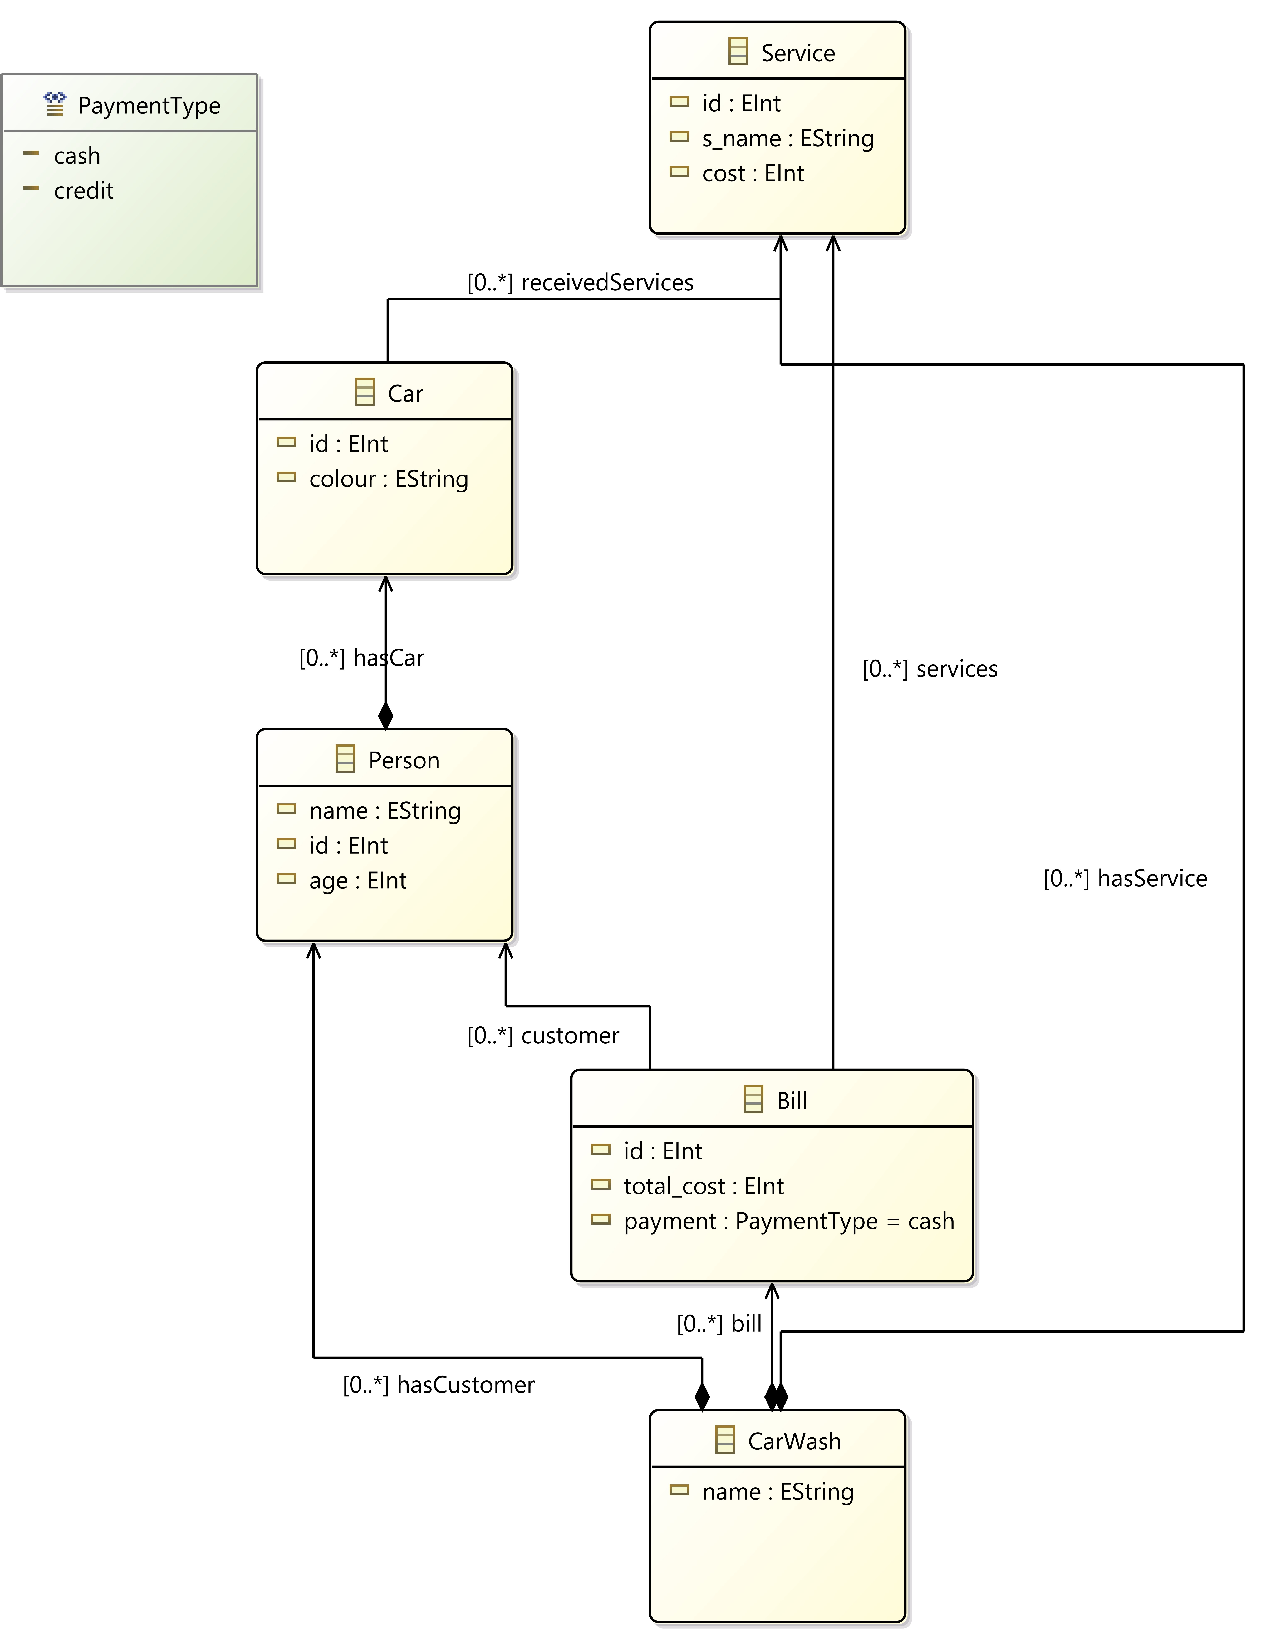
\includegraphics[width=10 cm, clip]{Figures/ecorecarwash.pdf}
    \caption{Carwash metamodel in~\cite{rahimi2023towards}.\label{fig:ecorecarwash}}
\end{figure}


\begin{program_}[H]
\footnotesize
\begin{verbatim}
{'directed': True, 'multigraph': True,
'graph': {}, 'nodes': [{'type': 'Bill', 'id': 0},
{'type': 'Bill', 'id': 1},
{'type': 'CarWash', 'id': 2},
{'type': 'Car', 'id': 3},
{'type': 'Car', 'id': 4},
{'type': 'Car', 'id': 5},
{'type': 'Person', 'id': 6},
{'type': 'Person', 'id': 7},
{'type': 'Service', 'id': 8},
{'type': 'Service', 'id': 9},
{'type': 'Service', 'id': 10}],
'links': [{'type': 'customer', 'source': 0,
'target': 6, 'key': 0},
{'type': 'services', 'source': 0,
'target': 8, 'key': 0},
{'type': 'services', 'source': 0,
'target': 10, 'key': 0},
{'type': 'customer', 'source': 1,
'target': 7, 'key': 0},
{'type': 'services', 'source': 1,
'target': 9, 'key': 0},
{'type': 'bill', 'source': 2,
'target': 0, 'key': 0},
{'type': 'bill', 'source': 2,
'target': 1, 'key': 0},
{'type': 'hasCustomer', 'source': 2,
'target': 6, 'key': 0},
{'type': 'hasCustomer', 'source': 2,
'target': 7, 'key': 0},
{'type': 'hasService', 'source': 2,
'target': 8, 'key': 0},
{'type': 'hasService', 'source': 2,
'target': 9, 'key': 0},
{'type': 'hasService', 'source': 2,
'target': 10, 'key': 0},
{'type': 'receivedServices', 'source': 3,
'target': 8, 'key': 0},
{'type': 'receivedServices', 'source': 4,
'target': 10, 'key': 0},
{'type': 'receivedServices', 'source': 5,
'target': 9, 'key': 0},
{'type': 'receivedServices', 'source': 5,
'target': 10, 'key': 0},
{'type': 'hasCar', 'source': 6,
'target': 3, 'key': 0},
{'type': 'hasCar', 'source': 7,
'target': 4, 'key': 0},
{'type': 'hasCar', 'source': 7,
'target': 5, 'key': 0}]}
\end{verbatim}
\caption{The graph data of Carwash instance model in~\cite{rahimi2023towards}.}
\label{Listing:NetworkXRahimi}
\end{program_}

\subsection{Experiment 3}
In this experiment, we compared the graph encoding capabilities of MoEGL with the approach presented by Miranda~\cite{miranda2024towards}, which used machine learning-backed methods to compute model views with Heterogeneous Graph Neural Networks (HGNNs). Miranda et al. aimed to simplify the integration of machine learning into Model-Driven Engineering (MDE) by encoding instance models conforming to an FSM metamodel into graphs using both NetworkX and Heterogeneous PyG. Their encoding approach was designed to automatically infer inter-model links while decoupling the contributions of view engineers and machine learning specialists.

For their evaluation, Miranda et al. presented a sample graph in Listing~\ref{Listing:NetworkXJames}, which was generated using NetworkX. This graph represents an FSM model with 3 Transition nodes, 4 State nodes, and 6 relationships between transitions and states. In order to validate MoEGL's ability to replicate this encoding, we applied MoEGL to the same FSM dataset and generated the equivalent graphs using both NetworkX and PyG.

Our results showed that MoEGL produced identical graphs to those presented by Miranda~\cite{miranda2024towards}, with the same number of Transition and State nodes and identical relationships between these nodes. Both MoEGL and Miranda's approach yielded exactly 3 Transition nodes, 4 State nodes, and 6 edges connecting them, which confirms that MoEGL can accurately capture the structural aspects of the model. The generated graphs were identical in terms of structure and node-edge relationships across both tools.

To verify the accuracy of our encoding, we printed the graph data produced by MoEGL and compared it directly with the data presented by Miranda et al. in Listing~\ref{Listing:NetworkXJames}. The outputs were structurally identical, proving that MoEGL successfully replicates the model-to-graph transformation presented by Miranda. Listing~\ref{Listing:NetworkXJames} serves as a representative example of the graph produced by MoEGL, and we can confirm that our approach generates an exact match in terms of node types, counts, and relationships.

In this section, we have opted not to present the detailed DSL configuration used to generate the graphs, as similar DSL structures were already extensively covered in previous examples. Instead, we focus on providing the output of a sample graph, demonstrating that MoEGL can generate equivalent graphs without the need for repetitive DSL details. By omitting these details, we aim to avoid redundancy while maintaining clarity in our findings.

In conclusion, this experiment demonstrates that MoEGL can seamlessly replicate the graph encoding approach used by Miranda et al. across both NetworkX and PyG. This validation shows that MoEGL provides the same structural fidelity as previous work, while offering the flexibility to integrate with various machine learning frameworks. Researchers and engineers can confidently use MoEGL to generate graph representations that are fully compatible with existing approaches, ensuring consistency and reliability in model-to-graph transformations for advanced machine learning tasks.


\begin{program_}[H]
\footnotesize
\begin{verbatim}
{
  "nodes": [
    {"type": "Transition", "id": 0},
    {"type": "Transition", "id": 1},
    {"type": "Transition", "id": 2},
    {"type": "State", "id": 3},
    {"type": "State", "id": 4},
    {"type": "State", "id": 5},
    {"type": "State", "id": 6}
  ],
  "links": [
    {"type": ("Transition", "source",
    "State"), "source": 0, "target": 3},
    {"type": ("Transition", "target",
    "State"), "source": 0, "target": 4},
    {"type": ("Transition", "source",
    "State"), "source": 1, "target": 4},
    {"type": ("Transition", "target",
    "State"), "source": 1, "target": 5},
    {"type": ("Transition", "source",
    "State"), "source": 2, "target": 5},
    {"type": ("Transition", "target",
    "State"), "source": 2, "target": 6}
  ]
}
\end{verbatim}
\caption{The graph data of the FSM instance model in~\cite{miranda2024towards}.}
\label{Listing:NetworkXJames}
\end{program_}



Table~\ref{tab:experimentations} presents the key properties of each model dataset and its corresponding graph that are used in the experiments. Specifically, the analysis reveals the count of models and elements within each model. Additionally, it provides the average number of references, along with the number of nodes and edges in the graph representation.
It is important to note that the number of nodes in the generated graphs is almost equal to the total number of elements and references in the original models because all the elements, references, and attributes are mapped to nodes in the final graph. The table numbers indicate that the graph transformation can accurately capture all the structural information present in the models by creating graph nodes for each element and reference during the mapping process.
The table omits the number of attributes for each element since attributes were not considered in the scope of these experiments (the three original encoders in related work did not consider attribute values). Therefore, the goal is to evaluate how effectively MoEGL can replicate existing model-to-graph encoding techniques based on the structural aspects of the models, without integrating any attribute-level information.
By providing a high-level overview of the key structural characteristics of each model dataset and graph in a consolidated manner, this table helps to better understand the different model transformation experimentations.

This evaluation strongly indicates the practical usefulness of our approach, as all the diverse transformations from prior literature can be replicated seamlessly. Researchers can now focus solely on their neural models, without concerning themselves with the complex encoding implementations.

The MoEGL's ability to express a wide range of encoders establishes its value for the MDE community in enabling novel graph-based techniques like GNNs on modeling languages and data.

\begin{table}[H]
\caption{Key properties of the experimentations' model datasets.\label{tab:experimentations}}
\begin{adjustwidth}{-\extralength}{0cm}
\centering
\small
\begin{tabularx}{\fulllength}{ccccc cc}
\toprule
\textbf{Experimentation} & \textbf{Input Models Type} & \textbf{Number of Models} & \textbf{Avg. Elements} & \textbf{Avg. References} & \textbf{Avg. Nodes} & \textbf{Avg. Edges} \\
\midrule
Exp. 1~\cite{lopez2022generating} & ecore & 500 & 34 & 42 & 80 & 85 \\
Exp. 2~\cite{rahimi2023towards} & xmi   & 10  & 10 & 50 & 60 & 100 \\
Exp. 3~\cite{miranda2024towards} & xmi   & 20  & 95 & 250 & 350 & 500 \\
\bottomrule
\end{tabularx}
\end{adjustwidth}
\end{table}


\subsection{Additional Experiment: Using Models in Graph-Learning Benchmarks}

In the main experimentation, we replaced existing encoders from the MDE community with MoEGL encoders. Here we focus on a well-known graph-learning benchmark from the ML community, based on a graph dataset. We show that the same ML task can be performed using a dataset of modeling artifacts and a MoEGL encoder. This way, we want to show that MoEGL enables tackling common graph learning problems using models.

We choose an existing graph dataset and create a metamodel representing the graphs. We programmatically translate graphs of the dataset into instances of such metamodel. We write a MoEGL configuration that encodes these models. Finally, we compare the result of the encoding to the original graphs in the dataset, aiming at obtaining the same graphs.
The AIDS dataset from TUDataset~\cite{morris2020tudataset} is chosen as it contains node/edge labels and attributes. The dataset contains 2000 virus-screening compound graphs. Each node contains attributes like position, charge, and a label for its symbol. There are 38 symbol types and 3 edge types. The AIDS metamodel in Figure~\ref{fig:aidsmetamodel} depicts the structure of the AIDS graphs.
The attribute values are stored in the node attributes vector. The model is converted to the NetworkX format using MoEGL. We compared the generated graph and the original graph and found that the encoded structure and attributes are the same.

We are aware that the experiment validity is hampered by a certain circularity (i.e. we create the metamodel and both the model-to-graph and graph-to-model transformation), but we believe it to be still a meaningful hint to the potential of broadening the applicability of MDE techniques to graph learning.

\begin{figure}[H]
    \centering
    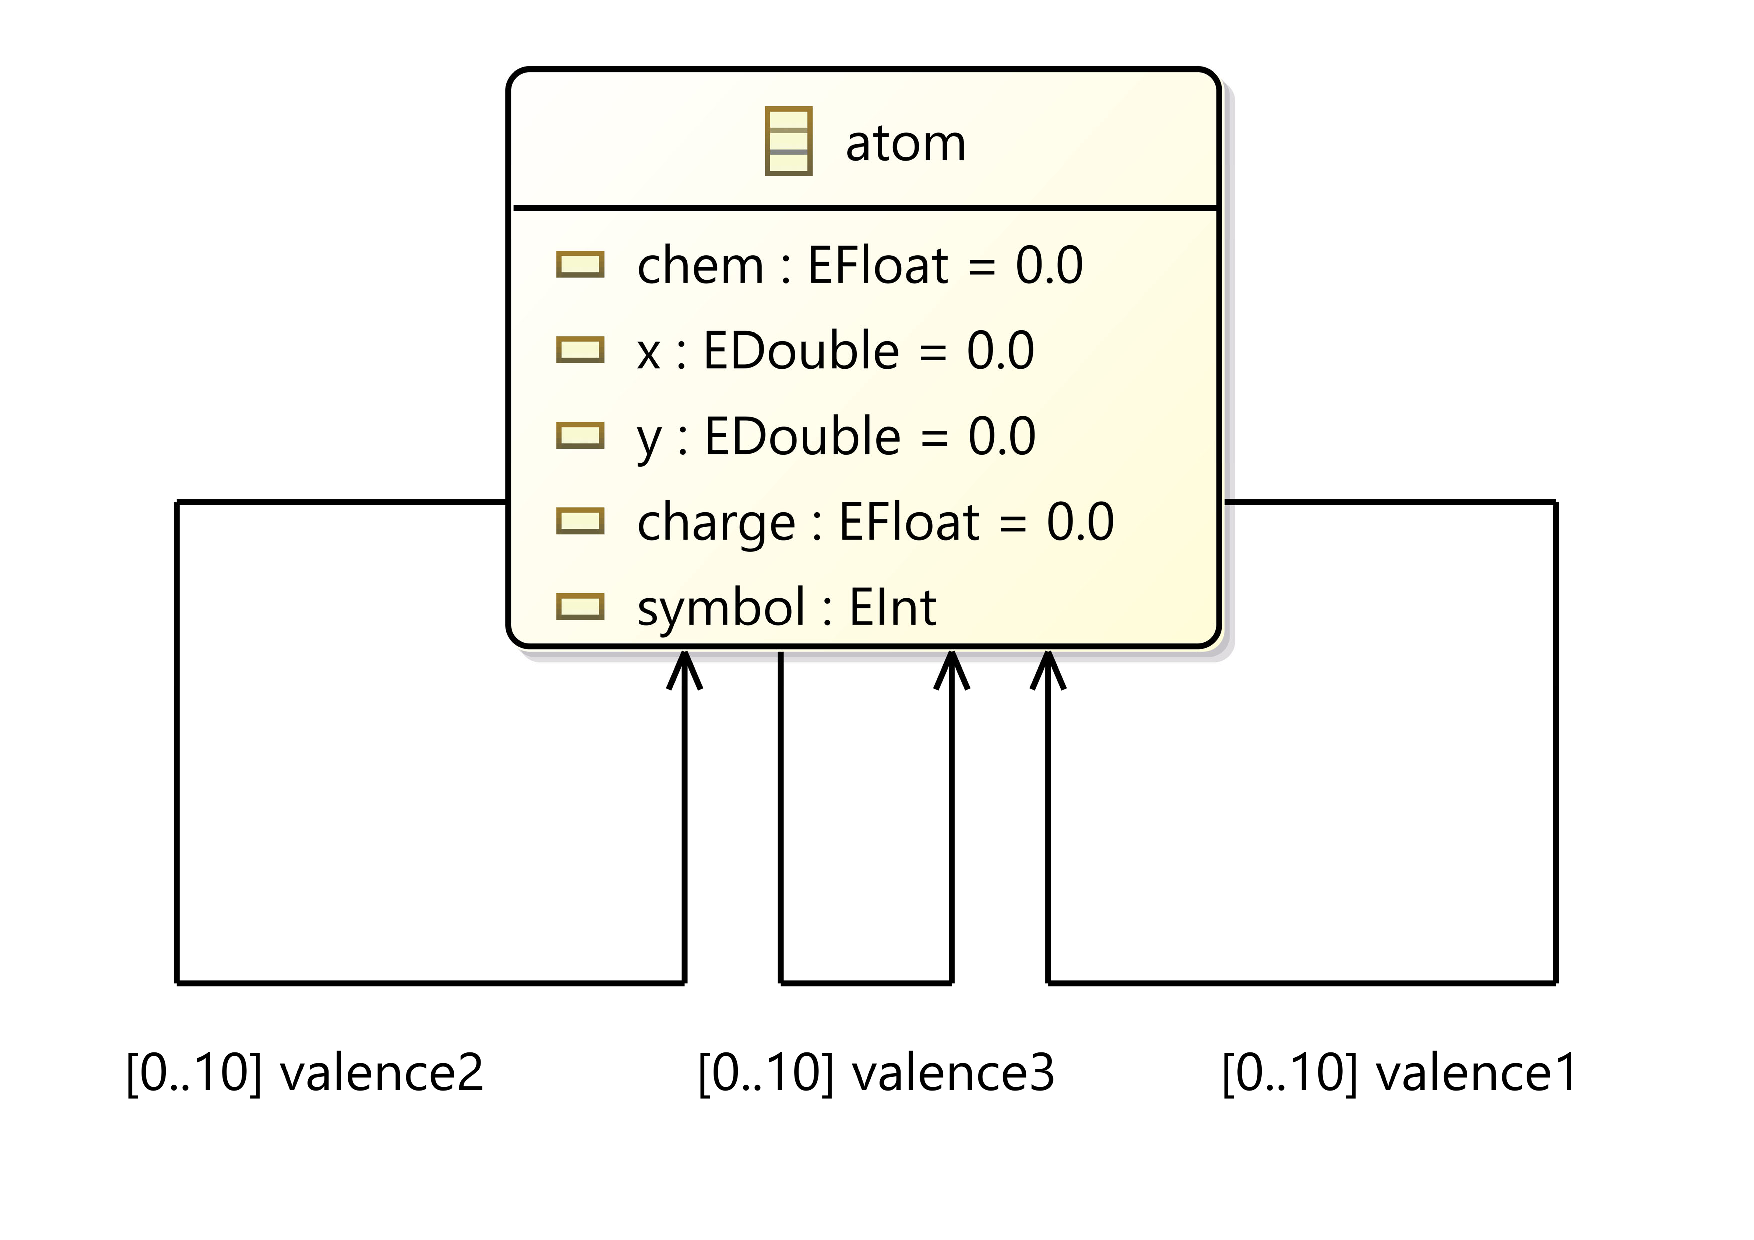
\includegraphics[width=10 cm]{Figures/AIDSmetamodel.pdf}
    \caption{The metamodel representing the graphs in the AIDS dataset.\label{fig:aidsmetamodel}}
\end{figure}

\subsection{Evaluation of MoEGL}

In this section, we evaluate the effectiveness of MoEGL in comparison to bespoke approaches. The evaluation focuses on both quantitative and qualitative metrics, providing a comprehensive assessment of how MoEGL improves the model-to-graph transformation process, particularly for developers working in Model-Driven Engineering (MDE) and utilizing Graph Neural Networks (GNNs).

\subsubsection{Quantitative and Qualitative Metrics}

To provide a thorough evaluation, we assess MoEGL across several key metrics:

\begin{itemize}
    \item \textbf{Time efficiency.} One of the major advantages of MoEGL is its ability to efficiently handle repeated transformations with different configurations. Once a model has been traversed and its elements extracted, subsequent encoding tasks with different DSL configurations can be completed in significantly less time. This is because the model data is already available, and MoEGL can reuse the extracted information without re-traversing the model. As a result, transformations such as adding or excluding specific node types, applying different encoding schemes, or modifying graph structures can be performed quickly. The times reported in Table~\ref{tab:evaluation} represent the average time required to transform 100 models. While the initial transformation time is comparable to bespoke approaches, subsequent transformations with different configurations are performed in a fraction of the time, offering substantial efficiency gains for iterative encoding tasks.

    \item \textbf{Lines of Code (LoC).} MoEGL's DSL drastically reduces the number of lines of code required for model-to-graph transformations. The DSL allows users to specify transformations declaratively, eliminating the need to write custom Python code for each transformation. This reduction in code complexity not only makes the solution more maintainable but also decreases the risk of coding errors. Table~\ref{tab:evaluation} demonstrates the significant reduction in LoC when using MoEGL.

    \item \textbf{Accuracy.} Both MoEGL and bespoke approaches generate identical graph structures in terms of nodes, edges, and relationships. MoEGL ensures that all structural information from the original models is accurately preserved during the transformation, providing 100\% accuracy, as confirmed by our experiments.

    \item \textbf{Scalability.} Scalability is a critical factor in evaluating model-to-graph transformations, especially as model sizes grow. MoEGL handles larger models more efficiently in terms of both execution time and memory usage. Table~\ref{tab:evaluation} shows that MoEGL performs better than bespoke approaches when processing larger datasets, making it a more scalable solution for complex MDE tasks.

    \item \textbf{Ease of Use.} MoEGL is designed to be user-friendly, enabling users with limited programming expertise to easily define transformations. Through user testing, we found that most users could quickly learn and apply MoEGL's DSL, resulting in significantly faster onboarding compared to writing custom Python scripts. This ease of use makes MoEGL accessible to a wider range of users, including domain experts who are not familiar with programming.

    \item \textbf{Maintainability.} The declarative nature of MoEGL's DSL enhances maintainability by allowing users to modify transformations without having to rewrite large portions of code. For example, users can easily add or exclude nodes and edges by updating the DSL configuration. This contrasts with bespoke approaches, where modifying transformations requires editing and testing complex Python code. MoEGL's simplified approach reduces maintenance overhead and minimizes the risk of introducing bugs during updates.

    \item \textbf{Extensibility.} MoEGL offers strong extensibility, allowing users to extend the DSL to support new node types, relationships, or attributes without significant modifications to the underlying system. This flexibility ensures that MoEGL remains adaptable to evolving model requirements. Bespoke approaches, in contrast, often require substantial refactoring to accommodate new features, making them less extensible in practice.
\end{itemize}

\subsection{Results Summary}

The table below summarizes the performance of MoEGL compared to bespoke approaches across the key metrics. The results clearly show that MoEGL improves time efficiency, reduces coding effort, and maintains high accuracy while offering better scalability, maintainability, and extensibility.

\begin{table}[H]
\caption{Comparison of MoEGL with Bespoke Approach based on Quantitative Metrics.\label{tab:evaluation}}
\begin{adjustwidth}{-\extralength}{0cm}
\centering
\begin{tabularx}{\fulllength}{lcc}
\toprule
\textbf{Metric}                   & \textbf{MoEGL (DSL)} & \textbf{Bespoke Approach} \\
\midrule
\textbf{Time Efficiency (s)}       & 2                 & 4.2                       \\
\textbf{Lines of Code (LoC)}       & 10                  & 85                        \\
\textbf{Accuracy}                  & 100\% identical     & 100\% identical           \\
\bottomrule
\end{tabularx}
\end{adjustwidth}
\end{table}

\noindent
The table highlights MoEGL's superior performance in terms of time efficiency, reduction in lines of code, and scalability. The accuracy of the graph transformations is identical for both MoEGL and bespoke approaches, ensuring reliability. In terms of qualitative metrics, user feedback indicates that MoEGL offers significantly improved ease of use, maintainability, and extensibility.


\section{Related Work} \label{Sec:relatedwork}
This section reviews some related studies that are proposed to do MDE tasks using ML models, especially those that exploit the model-to-graph encoding. However, MoEGL is the first one in the literature that does encoding, while considering desired constraints and multiple graph types.


ML algorithms have effectively tackled various challenges in MDE~\cite{babur2018ammore}. For instance, model transformation rules were automatically inferred from sets of source and target models using ML techniques in~\cite{burgueno2019lstm, dolques2010learning}. In~\cite{babur2016hierarchical}, a set of metamodels is arranged using hierarchical clustering to produce meaningful visualizations. Hierarchical clustering is also used in~\cite{basciani2016automated} to organize the models employing the MDEForge tool. There has also been a discussion on model encoding for clustering in~\cite{babur2017using}.
Nguyen et al.~\cite{nguyen2019automated} introduce a classification of metamodels by a tool implementing a feed-forward neural network. They propose some preprocessing tasks to transform a metamodel into a feature vector. The tasks consist of a term extractor that parses the terms in the meta-model, and then of an NLP Normalizer that normalizes the extracted terms by performing some Natural Language Processing (NLP) tasks. Burgueno et al.~\cite{burgueno2019lstm} propose a neural network architecture based on Long Short-Term Memory (LSTM) Neural Networks to perform model transformation automatically. They propose to apply a preprocessing method to represent models as trees before feeding them to an Artificial Neural Network (ANN). After transforming the model into a tree using the proposed strategy, a normalization process is applied to overcome the limitations of ANNs. Couto et al.~\cite{couto2020classifying} propose to classify unstructured models into meta-models using Multi-Layer Perceptrons (MLP). They translate a meta-model containing classes, attributes, and references into a set of name/value pairs in a JSON format. Then a binary vector is created as the MLP's input feature.

Some studies use model-to-graph encoding as their encoding approach. López et al.~\cite{lopez2021towards} address the issue of determining a generator's level of realism. They map it to a classification task where a GNN (GNN) will be trained to discriminate between the two sets of models (real and synthetic). In another study, López et al.~\cite{lopez2022generating} propose a new architecture for the design of structurally realistic generators. This kind of generator can create new models that are essentially novel but structurally similar to the models in the dataset given a dataset that includes multiple models considered real models. Graph kernels are suggested to be applied to MDE by the authors in~\cite{clariso2018applying}. Accordingly, Di Rocco et al.~\cite{di2021gnn} suggest MORGAN, a graph kernel-based tool to assist in the completion of models and metamodels. The tool's idea is to suggest structural elements to finish the models that are currently being built. Specifically, MORGAN can suggest metaclasses, structural elements like attributes and references, and classes, fields, and methods inside a model class.
Abbas et al.~\cite{rahimi2023towards} utilize generative adversarial networks (GANs) to automatically generate new structurally realistic models from a metamodel and instance model. The proposed GAN-based tool is built on the Eclipse Modeling Framework. Graph metrics are used to evaluate whether the generated artificial models match the properties of the original example model.
Miranda et al.~\cite{miranda2024towards} introduced the concept of model views to integrate heterogeneous models in MDE, the ViewPoint Definition Language (VPDL) for specifying model views, and the EMF Views solution. They have used an ML approach introduced to support automated link inference and HGNNs as the ML technique.

Clarisó and Cabot's work~\cite{clariso2022user} on user-driven diverse scenario exploration in model finders presents a domain-specific language (DSL) aimed at controlling how Alloy specifications are encoded into graphs for clustering purposes. Their DSL allows users to define scenarios by selecting and filtering model elements and attributes, providing a flexible approach to model exploration and analysis. This method, while targeting Alloy specifications, demonstrates the broader applicability and influence of DSLs in model-driven engineering. The concepts of selecting and filtering elements in their DSL are closely aligned with our approach, emphasizing the importance of user control and customization in model encoding processes. This highlights the versatility of DSLs in enhancing the usability and precision of model-driven tasks.

Each of these papers focuses on a specific learning task and encodes models according to its specific needs. By contrast, we do not focus on any specific task but rather propose a general encoding approach that aims to apply to any learning task.
The contribution of our work lies in leveraging graph learning frameworks and representing models as graphs. This approach enables us to exploit the capabilities of graph learning processes effectively. The most distinguishing feature of our approach is that it makes it relatively easy for users to specify their encoding preferences. All of the existing work apply a rough encoding process to the models and the encoding output is completely bonded to the input model.

\subsection{Schema Migration and Meta-Model Evolution}
Schema migration and meta-model evolution are central challenges in MDE, as changes in schemas or metamodels must be consistently propagated throughout models to avoid inconsistencies. Several approaches have been proposed to address these challenges. For instance, Kolovos et al.~\cite{kolovos2008detecting} proposed a technique for detecting and resolving inconsistencies caused by metamodel evolution in MDE environments. These works highlight the need for flexible and automated tools to manage model evolution, which MoEGL can contribute to by facilitating the encoding of models with evolving metamodels into graphs.

\subsection{Domain-Specific Transformation Languages (DSTLs)}
Domain-specific transformation languages (DSTLs) are tailored to specific domains and provide specialized syntax and semantics for model transformations. These languages aim to simplify the transformation process by focusing on domain-relevant tasks. For example, Varro et al.~\cite{csertan2002viatra} developed VIATRA, a DSTL aimed at transforming models for system verification. DSTLs are particularly useful in MDE for automating complex transformations, and MoEGL's DSL shares similar goals by enabling customizable model-to-graph encoding.


\section{Evaluation of Research Contributions and Questions}
In this section, we evaluate each of our research contributions and questions, demonstrating the strengths, limitations, and opportunities of our approach compared to others.

The main research contributions of the paper are:
\begin{itemize}
    \item \textbf{Introduction of MoEGL.} Strengths: MoEGL is the first domain-specific language (DSL) for encoding models into GNN-compatible graphs, addressing a critical gap in MDE. Opportunities: Future work can extend MoEGL to support more advanced encoding techniques and additional graph types.
    \item \textbf{Automated Encoding Process.} Strengths: The automated process significantly reduces manual effort and errors. Opportunities: Enhancements in UI and configuration tools can simplify the setup process.
    \item \textbf{Support for Heterogeneous Graphs.} Strengths: Accurately preserves structural and type information in MDE artifacts. Opportunities: Optimization techniques can be explored to handle larger models.
    \item \textbf{Empirical Validation.} Strengths: Experiments demonstrate MoEGL's practical utility and effectiveness. Opportunities: Broader testing across diverse models and MDE tasks can provide more comprehensive validation.
\end{itemize}

The main findings w.r.t. the outlined research questions are:
\begin{itemize}
    \item \textbf{Efficiency.} Findings: MoEGL significantly improves efficiency compared to manual approaches. Strengths: Automation streamlines workflow and minimizes human error. Opportunities: Further optimizations and parallel processing can enhance efficiency.
    \item \textbf{Usability.} Findings: Domain experts found MoEGL accessible and easy to use. Strengths: The DSL syntax is intuitive for non-programmers. Opportunities: Comprehensive documentation and tutorials can enhance usability.
    \item \textbf{Accuracy and Maintainability.} Findings: Produces highly accurate and maintainable graphs. Strengths: Generated graphs are consistent and reliable. Opportunities: Continuous refinement of algorithms based on user feedback.
    \item \textbf{Generalizability.} Findings: Performs well across different models and MDE tasks. Strengths: Versatility makes it a valuable tool for a wide range of applications. Opportunities: Expanding supported models and integrating with other tools can enhance generalizability.
\end{itemize}

By evaluating these contributions and questions, we have shown that MoEGL not only simplifies the model encoding process but also offers significant strengths and opportunities for further development. The limitations identified provide a clear direction for future research and improvements.


\section{Conclusion and Future Work} \label{Sec:conclusion}

In this paper, we introduced MoEGL, a domain-specific language designed to encode models into graphs compatible with graph neural networks. Our experiments demonstrate that MoEGL can effectively replace custom, manual encoding methods, providing a more streamlined and error-free approach to model encoding. Future work will explore further enhancements to MoEGL and its application to other MDE tasks.

By situating our work within the broader context of model-driven engineering and machine learning, we have shown that MoEGL addresses significant challenges identified in the literature, such as the need for automated, accurate, and flexible model encoding techniques. Our contributions build on and extend the research of Nguyen et al.~\cite{nguyen2019automated}, Osman et al.~\cite{osman2018automated}, and others, offering a robust solution that enhances the integration of GNNs in MDE.

In this work, we put forth a DSL called MoEGL (Model Encoding for Graph Learning) to encode models into graph-structured data to assist those in the MDE community in carrying out ML tasks on desired collections of models. MoEGL allows users to leverage their domain knowledge and preferences to make the encoding process more efficient. Specifically, MoEGL empowers users to filter any class or feature from the metamodel that should be excluded from the encoding. Additionally, users can specify the desired output graph format through the configuration of MoEGL. Our experimental findings demonstrate that the encoding generated by MoEGL successfully conveys all pertinent data contained within the models while preserving the structural relationships. By applying MoEGL, all salient details encompassed by the complex metamodels, including attributes and the semantics of connections between concepts, are represented accurately in the derived graph-based encoding. This facilitates downstream ML applications to extract useful insights from the encoded modeling data.

Looking ahead, we aim to further develop MoEGL to be sufficiently versatile that it can be applied to any Deep Learning tasks involving models. Some potential avenues of future work include considering alternate encodings for attribute values within MoEGL, allowing users to filter model elements according to Object Constraint Language (OCL) expressions defined in the MoEGL configuration, and more fully realizing the proposed heterogeneous graph encoding approach. A goal is to semantically encode the element names in models to facilitate various MDE activities. Another possible extension of this research going forward involves designing heuristics to automatically determine well-suited encodings based on analyzing a metamodel's structure and characterizing the ML objective. Moving ahead, we plan to extensively research the applicability of encoding models as heterogeneous graphs for a wide range of MDE use cases. We also intend to support other popular GNNs and HGNNs like the new implementation of heterogeneous graphs in tensorflow~\cite{HPyG_Tensorflow}. The potential benefits of our encoding methodology warrant significant investigation into how it can most optimally support both current and emerging model-centric AI applications.

%%%%%%%%%%%%%%%%%%%%%%%%%%%%%%%%%%%%%%%%%%
\vspace{6pt}

%%%%%%%%%%%%%%%%%%%%%%%%%%%%%%%%%%%%%%%%%%
%% optional
%\supplementary{The following supporting information can be downloaded at \linksupplementary{s1}, Figure S1: title; Table S1: title; Video S1: title.}

%%%%%%%%%%%%%%%%%%%%%%%%%%%%%%%%%%%%%%%%%%
\authorcontributions{Conceptualization, Z.R. and S.K.-R.; methodology, Z.R.; software, Z.R.; validation, Z.R., S.K.-R. and M.T.; formal analysis, Z.R.; investigation, Z.R.; resources, Z.R.; data curation, Z.R.; writing---original draft preparation, Z.R.; writing---review and editing, S.K.-R. and M.T.; visualization, Z.R.; supervision, S.K.-R. and M.T.; project administration, S.K.-R.; funding acquisition, S.K.-R. All authors have read and agreed to the published version of the manuscript.}

\funding{This research received no external funding.}

\institutionalreview{Not applicable.}

\informedconsent{Not applicable.}

\dataavailability{The source code and data presented in this study are openly available in the MoEGL repository at \url{https://github.com/Z-Rajaei/MoEGL}.}

\acknowledgments{During the preparation of this manuscript, the authors used generative AI tools (e.g., ChatGPT and GitHub Copilot) for language polishing and code assistance. The authors have reviewed and edited the output and take full responsibility for the content of this publication.}

\conflictsofinterest{The authors declare no conflicts of interest. The funders had no role in the design of the study; in the collection, analyses, or interpretation of data; in the writing of the manuscript; or in the decision to publish the results.}

%%%%%%%%%%%%%%%%%%%%%%%%%%%%%%%%%%%%%%%%%%
%% Optional
\abbreviations{Abbreviations}{%
The following abbreviations are used in this manuscript:\\

\noindent
\begin{tabular}{@{}ll}
MDE & Model-Driven Engineering\\
DSL & Domain-Specific Language\\
GNN & Graph Neural Network\\
HGNN & Heterogeneous Graph Neural Network\\
ML  & Machine Learning\\
AI  & Artificial Intelligence\\
EMF & Eclipse Modeling Framework\\
UML & Unified Modeling Language\\
XMI & XML Metadata Interchange\\
OCL & Object Constraint Language\\
GAN & Generative Adversarial Network\\
LSTM & Long Short-Term Memory\\
MLP & Multi-Layer Perceptron\\
NLP & Natural Language Processing\\
MoEGL & Model Encoding for Graph Learning\\
HPyG & Heterogeneous PyTorch Geometric\\
GCN & Graph Convolutional Network\\
GAT & Graph Attention Network\\
LoC & Lines of Code\\
DOI & Digital Object Identifier\\
CSV & Comma-Separated Values\\
FSM & Finite State Machine\\
URI & Uniform Resource Identifier\\
URL & Uniform Resource Locator\\
YAML & YAML Ain't Markup Language
\end{tabular}
}

%%%%%%%%%%%%%%%%%%%%%%%%%%%%%%%%%%%%%%%%%%
%% Optional
\appendixtitles{no} % Leave argument "no" if all appendix headings stay EMPTY (then no dot is printed after "Appendix A"). If the appendix sections contain a heading then change the argument to "yes".
\appendixstart
\appendix
\section[\appendixname~\thesection]{}

All appendix sections must be cited in the main text. In the appendices, figures, tables, etc., should be labeled starting with ``A'', e.g., Figure A1, Figure A2, etc.

%%%%%%%%%%%%%%%%%%%%%%%%%%%%%%%%%%%%%%%%%%
\begin{adjustwidth}{-\extralength}{0cm}

\reftitle{References}

%=====================================
% References, variant A: external bibliography
%=====================================
\bibliography{sn-bibliography}

%=====================================
% References, variant B: internal bibliography
%=====================================
% To use the internal bibliography, comment out the \bibliography line above
% and uncomment the thebibliography environment below, then add your bibitems.

%%%%%%%%%%%%%%%%%%%%%%%%%%%%%%%%%%%%%%%%%%
\PublishersNote{}
\end{adjustwidth}
\end{document}
